\documentclass[11pt]{article}
% We can write notes using the percent symbol!
% The first line above is to announce we are beginning a document, an article in this case, and we want the default font size to be 12pt
% \usepackage[utf8]{inputenc}
\usepackage[left=1.2in,top=.8in,right=1.2in,nohead,bottom=.5in]{geometry}
% This is a package to accept utf8 input.  I normally do not use it in my documents, but it was here by default in Overleaf.

\usepackage{amssymb,amsthm,amsmath}
\usepackage{commath,hyperref}
\usepackage{enumerate,xcolor}
\usepackage{natbib}
\usepackage{graphicx}
\usepackage{caption,setspace}
\usepackage{subcaption}
\DeclareMathOperator{\Tr}{Tr}
\newcommand{\dd}[1]{\mathrm{d}#1}
\newcommand{\E}{\mathbb{E}}
\newcommand{\Var}{\text{Var}}
\newcommand{\Cov}{\text{Cov}}
\newcommand{\X}{\mathcal{X}}
\newcommand{\B}{\mathcal{B}}
\newcommand\numberthis{\addtocounter{equation}{1}\tag{\theequation}}
% These three packages are from the American Mathematical Society and includes all of the important symbols and operations 
\usepackage{fullpage}
\usepackage{comment}
\usepackage[linesnumbered, ruled]{algorithm2e}
% By default, an article has some vary large margins to fit the smaller page format.  This allows us to use more standard margins.
\allowdisplaybreaks
\newtheorem{theorem}{Theorem}
\newtheorem{lemma}{Lemma}
\newtheorem{corollary}{Corollary}

\theoremstyle{remark}
\newtheorem{example}{Example}
\newtheorem{ass}{Assumption}
\newtheorem{remark}{Remark}
\setlength{\parskip}{0em}
\setlength{\parindent}{0in}
\renewcommand{\arraystretch}{1.5}

% This gives us a full line break when we write a new paragraph
% \usepackage[mathscr]{euscript}
% \usepackage{tikz}
% \newcommand*\circled[1]{\tikz[baseline=(char.base)]{
%             \node[shape=circle,draw,inner sep=2pt] (char) {#1};}}
% \newcommand{\indep}{\perp \!\!\! \perp}


\title{Globally-centered autocovariances in MCMC}

\author{
  Medha Agarwal \\
  Department of Mathematics and Statistics\\
  IIT Kanpur\\
  \texttt{medhaaga@iitk.ac.in} \and
 Dootika Vats \\
  Department of Mathematics and Statistics\\
  IIT Kanpur\\
  \texttt{dootika@iitk.ac.in}
}


\begin{document}

\maketitle


\onehalfspacing
\begin{abstract}
Autocovariances are the fundamental quantity in many features of Markov chain Monte Carlo (MCMC) simulations with autcorrelation function (ACF) plots being often used as a visual tool to ascertain the performance of a Markov chain. Unfortunately, for slow mixing Markov chains, the empirical autocovariance can highly underestimate the truth. For multiple chain MCMC sampling,  we propose a globally-centered estimate of the autocovariance that pools information from all Markov chains. We show the impact of these improved estimators in three aspects: (1) acf plots, (2) estimates of the Monte Carlo asymptotic covariance matrix, and (3) estimates of the effective sample size. 
\end{abstract}


% {\color{blue} Main things to change
% \begin{itemize}
%   \item I don't want to call this ``Replicated autocovariance'' or ``Replicated spectral variance''. I think ``Globally-centered autocovariance'' is more appropriate and self-explanatory. So we will have to go over the whole document and change this.

%   \item The contents are a bit messy right now, and I am having trouble organizing my thoughts. 

% \end{itemize}

% A rough outline of the organization
% \begin{enumerate}
%   \item Introduction, with a sneak peak at new plots. Change this example to a univariate mixture of Gaussians.:

%     Here, we will just explain the problem with the old ACF and what happens by using the new ACF. We will show a plot to illustrate the impact. Then we will summarize the three places this will have an impact: (1) ACF plots (2) estimators of the asymptotic variance-covariance matrix (3) estimating effective sample size.

%   \item Globally-centered autocovariance
%     \begin{itemize}
%       \item Theoretical soundness
%     \end{itemize}

%   \item Variance of Monte Carlo averages

%     Describe MC averages and CLT here and not before
%     \begin{itemize}
%       \item Globally-centered Spectral variance estimators
%       \begin{itemize}
%         \item Theoretical results
%         \item Fast implementation
%       \end{itemize}
%     \end{itemize}

%   \item Effective sample size

%   \item Examples

%   \item Discussion
%     \begin{itemize}
%       \item All plots have been made using the package:(name). The package can be found on GitHub.
%       \item One thing to discuss is that the new autocovariances can be used in the initial sequence estimators as well.
%     \end{itemize}

%   \item Appendix
%     \begin{itemize}
%       \item Proofs
%       \item ACF plots for other examples.
%     \end{itemize}

% \end{enumerate}
% }
% \newpage

\section{Introduction} \label{sec:intro}

The power of the modern personal computer has made it easy to run parallel Markov chain Monte Carlo (MCMC) implementations. This is particularly useful for slow mixing or multi-modal target distributions, where the starting points of the chains are spread over the state-space in order to capture characteristics of the target distribution more accurately. The output from $m$ parallel chains is then summarized, visually and quantitatively, to assess the empirical mixing properties of the chains and the quality of Monte Carlo estimators.

A key quantity of interest that drives MCMC output analysis is the autocovariance function (ACvF). From their use in autocorrelation plots to assessing Monte Carlo variability of estimates, to determining when to stop MCMC simulation, autocovariances drive many visual and quantitative inferences users make from MCMC output. However, tools on estimating ACvF are largely constructed for output from one MCMC chain. {\color{blue} a little bit more here}.

% Markov chain Monte Carlo (MCMC) is a sampling method used to obtain serially correlated realizations from a desired probability distribution when i.i.d. sampling is difficult. Due to this serial correlation in samples, a larger number of MCMC samples are required to make inferences about the target distribution as compared to the independent ones. Therefore, it becomes imperative for an MCMC practitioner to have an idea about the underlying dependence structure in the Markov chains. Autocovariance function (ACF) characterizes this dependence at a particular lag $k$. 

Let $F$ be the target distribution with mean $\mu$ defined on the set $\X \subseteq \mathbb{R}^p$ equipped with a countably generated Borel $\sigma$-field $\mathcal{B}(\X)$. For $s = 1, \dots, m$, let $\{X_{st}; \; t \in \mathbb{Z}\}$ be the $s^{th}$ $F$-Harris ergodic stationary Markov chain \citep[see][for definitions]{meyn:twee:2009} employed to learn characteristics about $F$.
% If $\bar{X} = n^{-1} \sum_{t=1}^{n}X_t$ , then with probability 1, $\bar{X} \to \mu_g$ as $n \to \infty$. \\
The process is covariance stationary so that
the ACvF at lag $k$ depends only on $k$ and is defined as 
%
\[
    \Upsilon(k) = \Cov_F(X_{s1}, X_{s\,1+k})= \mathbb{E}_F \left[(X_{s1} - \mu)(X_{s\,1+k} - \mu)^T \right]\,.
\]
Estimating $\Gamma(k)$ is critical to assessing the quality of the sampler and the quality of sample statistics. Let $\bar{X}_s = n^{-1} \sum_{t=1}^{n} X_{st}$ denote the Monte Carlo estimator of $\mu$ from the $s$th chain. The standard estimator for $\Gamma(k)$ is the sample autocovariance matrix at lag $k$. For the $s$th chain, it is given by
%
\begin{equation} \label{eq:empirical_ACvF}
    \hat{\Gamma}_s(k) = \dfrac{1}{n}\sum_{t=1}^{n-\abs{k}} \left(X_{st} - \bar{X}_s \right) \left(X_{s\, t+\abs{k}} - \bar{X}_s \right)^T\,.
\end{equation}
%
% It is a known fact that most of the Markov chains obtained from practical MCMC algorithms are not stationary. Regardless, Equation~\ref{eq:empirical_ACvF} provides the empirical estimator for ACF at a particular lag for the Markov chain with any initial distribution (\cite{geyer2011introduction}).\\

% Calculation of exact ACF has been done for simple stationary stochastic models like autoregressive (AR) models (under assumption of stationarity), moving average (MA) (\cite{quenouille1947notes}), and autoregressive-moving-average (ARMA) (\cite{box2015time}) models. However, for most of the complex sampling algorithms (including MCMC), we rely on sample estimators for ACF. Unfortunately, the estimator given in Equation~\ref{eq:empirical_ACvF} has been observed to have a some drawbacks. Firstly, it is not immune to outliers (see \cite{ma2000highly}) and secondly, it is usually non-informative in case of slowly mixing Markov chains. 
For single-chain MCMC runs, the estimator $\hat{\Gamma}(k)$ is used to construct autocorrelation (ACF) plots, to estimate the long-run variance of Monte Carlo estimators \cite{hannan:1970,dame:1991}, and to estimate effective sample size for an estimation problem \cite{kass:carlin:gelman:neal:1998,gong:fleg:2016,vats:fleg:jon:2019}. 

However, there is no unified approach to constructing estimators of $\Gamma(k)$ for multiple-chain implementations. Specifically, parallel MCMC chains are often spread across the state space so as to adequately capture high density areas. For slow mixing Markov chains and multi-modal targets, the chains take time to traverse the space so that estimates of $\mu$ can be vastly different. The sample ACvF from each chain is typically underestimated yielding false sense of security about the quality of process.

% We address the second issue in this paper by using multiple representative samples of the target distribution via parallel Markov chains. This approach is especially relevant to MCMC wherein multiple chain sampling is computationally possible and statistically desirable for making informative inferences. Our goal is to pool in the information from all the Markov chains while estimating the autocovariances. 

 % A commonly faced problem with the MCMC models is the slow mixing property. Especially in case of multi modal target distributions, it has been observed that the Markov chains tend to get \textit{stuck} in a particular mode for a long time. In such situations, single chain empirical ACF will severely underestimate the autocovariance. 
 We propose a globally-centered ACvF (G-ACvF) that centers the Markov chain around the overall mean vector from all $m$ chains. We show that the bias under stationarity for G-ACvF is lower than $\hat{\Gamma}(k)$, and through various examples, empirically demonstrate improved estimation. We employ the G-ACvF estimators to construct autocorrelation plots, which leads to remarkable improvements. A demonstrative example is at the end of this Section. 


% We will further study the impact of G-ACF in calculation of two important applications of ACF (1) asymptotic variance of Markov chain average and (2) effective sample size (ESS).
 
ACvFs are required to estimate the long-run variance of Monte Carlo averages. Specifically, spectral variance estimators are used to estimate $\Sigma = \sum_{k=-\infty}^{\infty} \Gamma(k)$. We replace $\hat{\Gamma}(k)$ with G-ACvF in spectral variance estimators (SVE) and show strong consistency of this estimator under weak conditions. In the spirit of \cite{andr:1991}, we also obtain large-sample bias and variance of the resulting estimator of $\Sigma$. Spectral variance estimators can be slow to prohibitively expensive to calculate \citep{liu:fleg:2018}. To relieve the computational burden, we adapt the fast algorithm of \cite{heberle2017fast} for G-ACvFs that dramatically reduces computation time. The globally-centered spectral variance estimator (G-SVE) is employed in the computation of effective sample size through the estimator given by \cite{vats2019multivariate}. We will show that using G-SVE for estimating $\Sigma$ safeguards us against early termination of the MCMC process and improves the reliability of estimators. 


% Let $g: \X \to \mathbb{R}^d$ be an F-integrable function and suppose we are interested in estimating the expected value $\mu_g = \mathbb{E}_F[g(X)]$. We know that $\sum_{t=1}^{n}g(X_t)/n$ converges to $\mu_g$ as $n \to \infty$ almost surely. MCMC ensures asymptotic convergence, however this is not practically very useful where the number of samples is finite and the Markov chain mixes slowly. 
% One of the important criteria to determine the quality of estimation is the Monte Carlo aymptotic covariance matrix which is given by an infinite summation of autocovariance matrices for all lags. For a slowly mixing Markov chain, underestimated autocovariances will deliver underestimated asymptotic variance. There are many techniques for estimating it like batch means (BM), overlapping bath means (OBM), and spectral variance estimator (SVE). Due to its nice statistical properties, we will only focus on SVE in this paper. SVE involves a truncated and weighted sum of autocovariances. We propose a version of SVE that uses our globally centered autocovariances. We call this globally-centered SVE (G-SVE).

% A more powerful estimator of Monte Carlo variability can enable us to estimate the effective sample size for the Markov chain which is closer to reality. There are many criteria for terminating simulation like fixed-time rule, sequencial fixed-volume rule (see \cite{glynn1992asymptotic}), and using Gelman Rubin diagnostics (\cite{gelman1992inference}). The relative fixed-volume rule has been thoroughly discussed for MCMC by \cite{flegal2015relative} and \cite{gong2016practical}. We will use method of effective sample size (ESS) by \cite{vats2019multivariate} for terminating the simulations. The quality of estimation of asymptotic covariance matrix is critical in estimation of the ESS. We will successfully show that the G-SVE estimates the truth better and prevents the premature stopping of Markov chain.

% The rest of the paper is arranged as follows. In Section~\ref{sec:G-ACF} we introduce the new sample autocovariance estimator and calculate its bias for finite samples. We observe that the bias term for G-ACF is similar to the bias of empirical ACF except for a few small order end-effect terms that vanish as $n \to \infty$. In Section~\ref{sec:variance_est}, we introduce the globally-centered SVE and give a proof of strong consistency, bias, and variance calculations. We will elaborate on the estimator for ESS using G-SVE in Section~\ref{sec:ess}. Section~\ref{sec:examples} gives an experimental study on three different examples for the proposed estimators. All the important proofs are given in the Appendix. 

\subsection{Demonstrative example} % (fold)
\label{sub:demonstrative_example}

% subsection demonstrative_example (end)
% \begin{example}[Demonstrative example]

We demonstrate the striking difference in estimation of $\Gamma(k)$ via autocorrelation function (ACrF) plots. Consider a random-walk Metropolis-Hastings sampler for a univariate mixture of Gaussians target density. Let the target density be 
\[
f(x) = 0.7\,f(x; -5, 1) + 0.3\,f(x; 5, 0.5)\,,
\]
where $f(x; a,b)$ is the density of a normal distribution with mean $a$ and variance $b$. 
Two Markov chains are started at each mode. Let $n$ denote the number of samples for each chain. Figure~\ref{fig:gaussian-trace} indicates that in the first $10^4$ samples, the chains do not jump modes so that both Markov chains yield different estimates of the population mean, $\mu$. At $10^5$ sample size, both Markov chains have traversed the state space reasonably and yield similar estimates of $\mu$. We make two points here: first, for small sample size, we observe that the locally-centered ACF gives misleading estimates whereas G-ACF accounts for the discrepancy in sample means between two chains. This is evident from the ACF plots  in Figure~\ref{subfig:gauss-acf}. Second, for a large sample size, the estimates from G-ACrF as well as ACrF are equivalent. Therefore, G-ACF can be used in any situation with a promise of estimates that are at least as good as empirical ACF estimators.  

\begin{figure}[htbp]
    \begin{subfigure}{.5\textwidth}
   \centering
   \includegraphics[width=\linewidth]{plots/gaussian-Targettrace_n1e4.pdf}
   \caption{$n = 10^4$}
   \label{subfig:gauss-trace_1e4}
 \end{subfigure}
 \begin{subfigure}{0.5\textwidth}
   \centering
   \includegraphics[width=\linewidth]{plots/gaussian-Targettrace_n1e5.pdf} 
   \caption{$n = 10^5$}
   \label{subfig:gauss-trace_1e5}
 \end{subfigure}
    \caption{Target density and trace plots for two chains starting at different values.}
    \label{fig:gaussian-trace}
\end{figure}



\begin{figure}[htbp]
\centering
\begin{subfigure}{.9\textwidth}
   \centering
   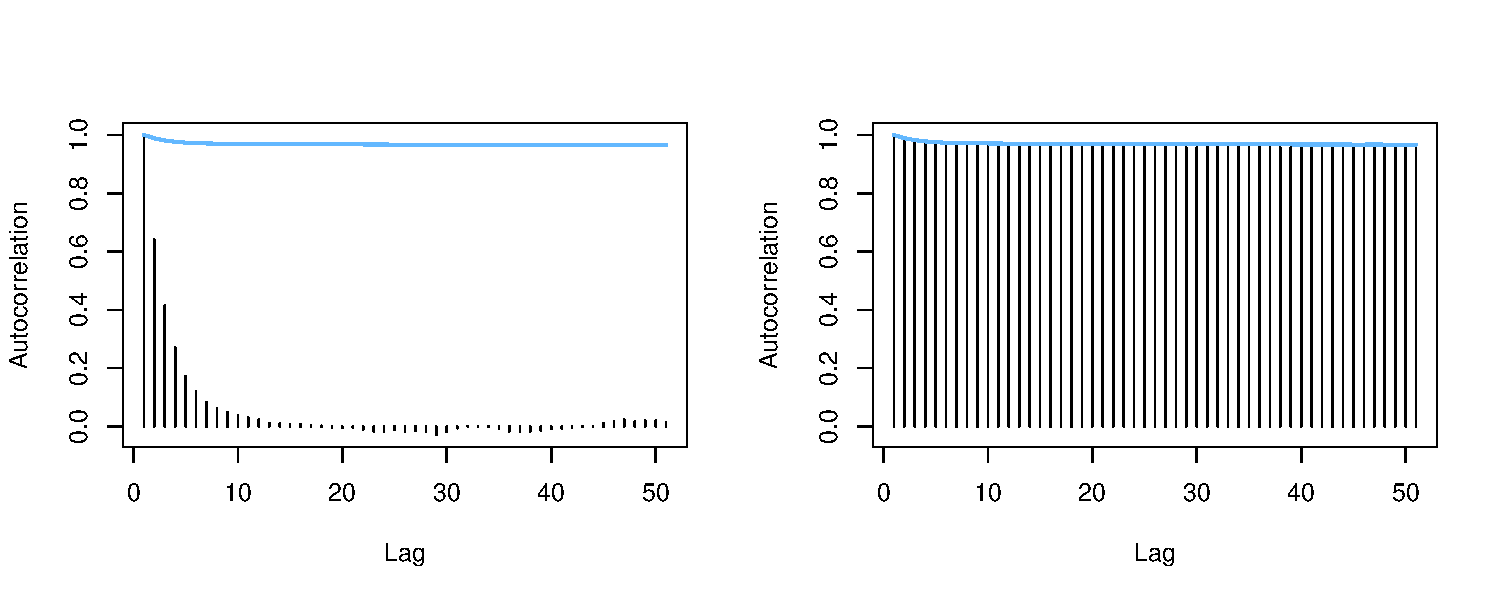
\includegraphics[width=.9\textwidth]{plots/gaussian-acf_hist.pdf}
   \caption{$n-10^4$ (histogram) and $n = 5 \times 10^5$ (blue line)}
   \label{subfig:gauss-acf_1e4_1e5}
\end{subfigure}
\begin{subfigure}{.9\textwidth}
   \centering
   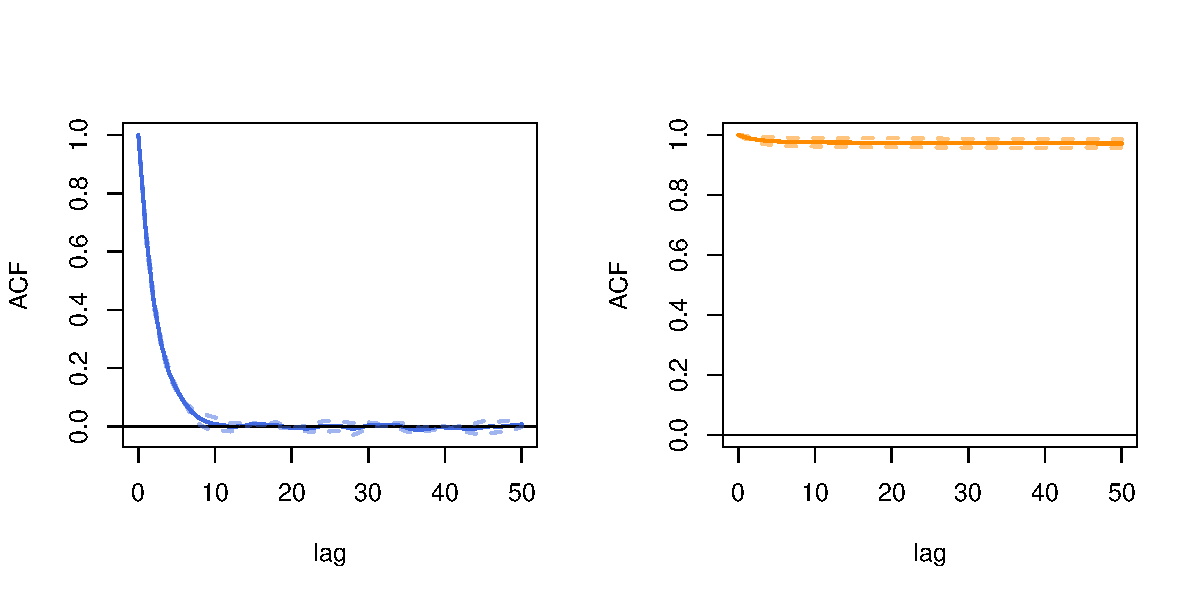
\includegraphics[width=.9\textwidth]{plots/gaussian-acf_1e4.pdf} 
   \caption{$n = 10^4$}
   \label{subfig:gauss-acf_1e4}
\end{subfigure}
\caption{ACF plots for locally-centered ACF (left) and globally centered ACF (right). (a) The histogram plots the estimates for $n = 10^4$ and the blue line plot the estimates for $n = 5 \times 10^4$ for chain-1. (b) $n = 10^4$; the dotted lines are ACF for each chain and the thick solid line is the ACF averaged over both chains.}
\label{fig:gaussian-acf}
\end{figure}


\section{Globally-centered autocovariance} \label{sec:G-ACF}

Recall that we run $m$ independent $F$-ergodic Markov chains denoted by $\{X_{st}; \; t \in \mathbb{Z}\}$ for the $s^{th}$ chain. Let the sample mean of the $s^{th}$ Markov chain be $\bar{X}_s = n^{-1} \sum_{t=1}^{n} X_{st}$ and the global mean by $\bar{\bar{X}} = m^{-1}\sum_{s = 1}^{m}\bar{X}_s$. The global mean is naturally superior estimator of $\mu$ than $\bar{X}_s$. We define the globally-centered autocovariance function (G-ACvF) estimator for the $s^{th}$ Markov chain as
%
\begin{equation} \label{eq:G-ACvF}
    \hat{\Gamma}_{G,s}(k) = \dfrac{1}{n} \sum_{t=1}^{n-k}(X_{st}-\bar{\bar{X}})(X_{s(t+k)}-\bar{\bar{X}})^T,
\end{equation}

In the event that all $m$ Markov chains have been run long enough that $\bar{X}_s \approx \bar{\bar{X}}$ are similar, then  $\hat{\Gamma}_{s} (k) \approx \hat{\Gamma}_{G,s}(k)$. However, for shorter runs or for slow mixing chains, $\Gamma(k)$ is more appropriately estimated by $\hat{\Gamma}_{G,s}$ as it utilizes information from all chains and accounts for disparity between estimates of $\mu$. We quantify the gains in  bias  for the G-ACvF estimator below.
% If the starting points of these parallel Markov chains are sufficiently dispersed, G-ACF provides more realistic estimation of lag covariances. \cite{priestley1981spectral} shows that the empirical estimator in Equation \ref{eq:empirical_ACvF} is biased with the main bias term equal to $\abs{k}\Gamma(k)/n$, ignoring the small order terms arising due to estimation of $\mu$. Though, an unbiased estimator with a divisor of $n - \abs{k}$ instead of $n$ exists, the biased estimator is preferred for its lower mean square error for larger relative $k$  (\cite{priestley1981spectral})
Let 
\[
\Phi^{(q)} = \sum_{ k= -\infty}^{\infty}\abs{k}^q \Gamma(k)\,,
\]
and let $\Phi^{(1)}$ be denoted by $\Phi$.  The proof of the following theorem is available in Appendix~\ref{appendix:bias}.

\begin{theorem} \label{th:G-ACF_bias} Let $\E_F \|X_{11}\|^{2 + \delta} < \infty$ for some $\delta > 0$. Let $P$ be a  polynomially ergodic Markov chain of order $\xi > (2 + \epsilon)/(1 + 2/\delta)$ for some $\epsilon > 0$. Then,
\[
   \mathbb{E}_F\left[\hat{\Gamma}_{G,s}(k) \right] = \left(1- \dfrac{|k|}{n}\right) \left(\Gamma(k) - \dfrac{\Sigma}{mn} - \dfrac{\Phi}{mn^2}\right)  + o \left(n^{-2} \right)\,,
\]
and consequently,
\[
\mathbb{E}_F\left[\hat{\Gamma}_{G,s}(k) - \hat{\Gamma}_s(k) \right] =  \left(1- \dfrac{|k|}{n}\right)\left(1- \dfrac{1}{m}\right)\left(\dfrac{\Sigma}{n} + \dfrac{\Phi}{n^2}\right) + o\left(n^{-2} \right)\,. 
\]
\end{theorem}

{\color{orange}MA: I corrected the RHS for the abover equation. Or did you mean to write $\mathbb{E}_F\left[\hat{\Gamma}_{G,s}(k) - \Gamma(k) \right]as LHS?$} 

\begin{remark}
Polynomial ergodicity and the moment conditions are required to ensure $\Phi$ and $\Sigma$ are finite. The above result can be stated more generally for $\alpha$-mixing processes, but we limit our attention to Markov chains. 
\end{remark}


When $m = 1$, $\hat{\Gamma}_{G,s}(k) = \hat{\Gamma}_{s}(k)
$ the bias results for which can be found in \cite{priestley1981spectral}. Since lag-covariances are typically positive in MCMC, Theorem~\ref{th:G-ACF_bias} implies that the G-ACvF estimators are asymptotically unbiased and exhibit reduced bias in finite samples compared to locally-centered ACvF estimators. The consequences of this are particularly pertinent for the diagonals of $\Gamma(k)$.
 % Special interest is also in the lag-0 autocovariance, that is, the variance of the target distribution. 
\begin{remark} \label{rem:lag0_expectation}
The variance of the target distribution is the lag covariance at lag 0 and is of particular interest. The bias of the estimator reduces by a factor of $m$:
\[
\mathbb{E} \left[\hat{\Gamma}_{G}(0) \right] = \Gamma(0) - \dfrac{\Sigma}{mn} - \dfrac{\Phi}{mn^2} + o(n^{-2})
\]
\end{remark}



A first use of the ACvFs in MCMC is in constructing ACF plots. Let the target variance of $i${th} component be $\Gamma^{ii}(0)$. For any component $i$, the autocorrelation is defined as
\[
\rho^{ii}(k) = \dfrac{\Gamma^{ii}(k)}{\Gamma^{ii}(0)}\,,
\]
and is instrumental in visualizing the serial correlation in components of the Markov chain. The typical estimate of the autocorrelation is constructed from $\hat{\Gamma}_s(k)$. Instead, we advocate for using G-ACvF estimates so that,
\[
\hat{\rho}_{G,s}^{(i)}(k) = \dfrac{ \hat{\Gamma}^{(i)}_{G,s} (k)}{\hat{\Gamma}^{(i)}_{G,s} (0)}.
\]
The globally-centered autocorrelation provides a far more realistic assessment of the correlation structure of marginal components of the chain  as evidenced in Figure~\ref{fig:gaussian:acf}. 

We end this section by noting that we can obtain an average G-ACvF and G-ACF over all $m$ chains
\[
\hat{\Gamma}_G(k) = \dfrac{1}{m}\sum_{s=1}^m \hat{\Gamma}_{G,s}(k) \quad \text{ and } \quad \hat{\rho}^{(i)}_G(k) = \dfrac{1}{m}\sum_{s=1}^m \hat{\rho}^{(i)}_{G,s}(k)\,.
\]
The averaged estimators present a measure of the overall correlation structure induced by the Markov transition $P$. 

\section{Variance estimators for multiple Markov chains} \label{sec:variance_est}

A critical use of autocovariances is in the assessment of Monte Carlo variability of estimators.  Let $g:\X \longrightarrow \mathbb{R}^p$ be an $F$-integrable function so that interest is in estimating
%
\[
\mu_g = \mathbb{E}_F[g(X)] = \int_{\X}g(x)F(dx)\;.
\]
 
Set $\{Y_{st}\}_{t \geq 1} = \{g(X_{st})\}_{t \geq 1}$ for all $s = 1, \dots, m$. Let $\bar{Y}_s = n^{-1}\sum_{t=1}^{n}Y_{st}$  and  $\bar{\bar{Y}} = m^{-1}\sum_{s=1}^{m}\bar{Y}_s$. By Birkhoff's ergodic theorem,  $\bar{\bar{Y}} \to \mu_g$ as $n \to \infty$ with probability 1.

Reliability of $\bar{\bar{Y}}$ is assessed by its Monte Carlo variability via an asymptotic sampling distribution \citep{fleg:hara:jone:2008,roy:2019,vats:rob:fle:jon:2020}. 
% To assess the reliability of simulations, we are interested in Monte Carlo error, i.e. $\bar{Y_s} - \mu$ for the $s^{th}$ chain. 
% The sampling distribution for Monte Carlo error is available via Markov chain CLT (\cite{jones2004markov})
 A Markov chain central limit theorem (CLT) holds if there exists a $p \times p$ positive-definite matrix $\Sigma$ such that
%
\begin{equation}
\label{eq:CLT}
  \sqrt{mn}(\bar{\bar{Y}} - \mu_g) \xrightarrow{d} N(0,\Sigma)\,
\end{equation}
where
\begin{equation}
\label{eq:sigma}
  \Sigma = \sum_{k = -\infty}^{\infty} \Cov_F \left( Y_{11}, Y_{1(1+k)} \right) := \sum_{k = -\infty}^{\infty}\Upsilon (k)
\end{equation}
%
The goal in output analysis for MCMC is to estimate $\Sigma$ in order to assess variability in $\bar{\bar{Y}}$. There is a rich literature on estimators of $\Sigma$ available for single-chain MCMC implementations. The most common are spectral variance estimators (SVE) \citep{andr:1991,vats:fleg:jon:2018} and batch means estimators \citep{chen:seila:1987,vats:fleg:jon:2019}. Recently, \cite{gupta:vats:2020} constructed a replicated batch means estimator for estimating $\Sigma$ from multiple parallel chains. Batch means estimators are computationally more efficient than SVE, whereas SVE estimators are more reliable \citep{fleg:jone:2010}. Here, we utilize G-ACvF estimators to construct globally-centered SV estimator (G-SVE) of $\Sigma$. Using the methods of \cite{heberle2017fast}, we also provide an efficient algorithm for obtaining the G-SV estimator. 

SV estimators are constructed as weighted and truncated sums of estimated lag covariances. The locally and globally centered empirical estimators for $\Upsilon(k)$, $\hat{\Upsilon}_s(k)$ and $\hat{\Upsilon}_{G,s}(k)$, can be defined in a similar way as $\hat{\Gamma}_s$ and $\hat{\Gamma}_{G,s}$ in Equation~\ref{eq:empirical_ACvF},\ref{eq:G-ACvF} for the Markov chain $\{Y_{st}\}_{t \geq 1}$ for all $s$. Let $w: \mathbb{R} \to [-c,c]$ be a lag window function and $b_n \in \mathbb{N}$ be a truncation point. The SV estimator of $\Sigma$ from a single chain is
%

\begin{equation} \label{eq:sve}
    \hat{\Sigma}_{s} = \sum_{k=-n+1}^{n-1}w\left(\dfrac{k}{b_n}\right)\hat{\Upsilon}_s(k)
\end{equation}

An overall estimate of $\Sigma$ from all $m$ chains is the average SV estimator (ASV):
\[
\hat{\Sigma}_A = \dfrac{1}{m}\sum_{s=1}^{m}\hat{\Sigma}_{s}\;.
\]
%  We propose a globally-centered spectral variance estimator (G-SVE) wherein we use G-ACF to estimate the autocovariance. Strong consistency for MSVE has been addressed by \cite{vats:fleg:jon:2018}. Bias and variance calculations for a variant of SVE with known mean is done by \cite{hannan2009multiple}. In this paper, we will address the asymptotic properties (strong consistency), bias and variance calculations for G-SVE. 

\subsection{Globally-centered spectral variance estimators} % (fold)
\label{sub:globally_centered_spectral_variance_estimators}

% subsection globally_centered_spectral_variance_estimators (end)

% Recall from Equation \ref{eq:empirical_ACvF} that $\hat{\Gamma}(k)$ is the empirical autocovariance function given by 

% \begin{equation}
%     \hat{\Gamma}(k) = \dfrac{1}{n}\sum_{t=1}^{n-\abs{k}}(X_t - \bar{X})(X_{t + \abs{k}} - \bar{X})^T
% \end{equation}

We define the globally-centered SV estimator as the weighted and truncated sum of G-ACvFs
%
% Consider $m$ Markov chains where $\hat{\Gamma}_s(k)$, $\hat{\Gamma}_{G,s}(k)$ and $\hat{\Sigma}_{S, s}$ are the lag-$k$ empirical ACF, G-ACF, and SVE respectively for $s^{th}$ Markov chain, $s\in {1,...,m}$. 
% Consider the globally-centered SV estimator (G-SVE) for the $s$th chain using G-ACF:
%
\begin{align*}
    \hat{\Sigma}_{G} &= \sum_{k=-b_n+1}^{b_n-1}w\left(\dfrac{k}{b_n}\right)\hat{\Upsilon}_{G}(k)\,.
\end{align*}
% and the combined G-SVE is
% \[
% \hat{\Sigma}_{G} =  \dfrac{1}{m}\sum_{s=1}^{m}\hat{\Sigma}_{G,s}\,.
% \]
For $\hat{\Sigma}_{G}$ to accurately estimate $\Sigma$, conditions need to be imposed on the weight function, $w$. 
%

\begin{ass}
\label{ass:lag_window}
The lag window $w(x)$ is a continuous at $0$ and at all but finite number of points. It is bounded and even function with $w(0)=1, \; \abs{w(x)} < c$, \; $\int_{-\infty}^{\infty}w^2(x)dx < \infty$, and $W = \sum_{k = -\infty}^{\infty} w(k/b_n)$ is finite.
\end{ass}
% We will consider a range of lag windows $w(x)$; where $w(x)$ is a continuous, even function with $w(0)=1, \abs{w(x)} < c$, $\int_{-\infty}^{\infty}w^2(x)dx < \infty$, and $W_n < \infty$. 
Assumption~\ref{ass:lag_window} is standard \citep[see]{ande:1971} and is satisfied by most lag windows. We will use the popular Bartlett lag window in our simulations. The function $w(.)$ is given by
\[
w(x) = \begin{cases}
\left(1 - \abs{x}\right) & \textrm{for } \abs{x} \leq 1 \\
0 & \textrm{otherwise}\,.
\end{cases}
\]

In relation to lag window, we are interested in $w(k/b_n)$ for lag-$k$. Therefore, zero weightage is given to autocovariances for lag greater than the truncation point $b_n$. This is true for Bartlett but not true for the quadratic spectral lag window in \cite{andr:1991} for example.

\subsubsection{Theoretical results} \label{sec:G-SVE}

We will present three main results for the G-SV estimator. First, we provide conditions for strong consistency. Strong consistency is particularly important to demonstrate for MCMC as it is required to ensure sequential stopping rules yield correct coverage at termination \citep{glyn:whit:1992}. A critical assumption is that of a strong invariance principle below. Let $B(n)$ denotes a standard $p$-dimensional Brownian motion.


\begin{theorem}[\cite{kuel:1976,vats:fleg:jon:2018}]
  \label{thm:kuelbs}
Let $\E_F\|Y_{11}\|^{2+ \delta} < \infty$ for $\delta > 0$ and let $P$ be a polynomially ergodic Markov chain of order $\xi > (q + 1 + \epsilon)/(1 + 2/\delta)$ for $q \geq 1$. Then there exists a $p \times p$ lower triangular matrix $L$ such that $LL^T = \Sigma$, a non-negative function $\psi(n) = n^{1/2 - \lambda}$ for some $\lambda > 0$, a finite random variable $D$, and a sufficiently rich probability space $\Omega$ such that for almost all $\omega \in \Omega$ such that for all $n > n_0$, with probability 1,
\[
\left\|\sum_{t=1}^{n}Y_t - n\mu_g - LB(n)\right\| < D\psi(n)\,.
\]
\end{theorem}

% \begin{ass}[Strong Invariance Principle (SIP)] \label{ass:sip}
%     We assume the SIP holds for the Markov chains $\{Y_{st}\}_{t \geq 1} \; \forall s$. Here $\{Y_t\}_{t\geq 1}$ is the stochastic process that follows SIP with mean $\mu_g$. Let $\|.\|$ denote the Euclidean norm. Through SIP, there exists a $p \times p$ lower triangular matrix L, an increasing function $\psi$ on the integers, a finite random variable D, and a  sufficiently rich probability space such that, with probability 1, \\
%   $$\left\|\sum_{t=1}^{n}Y_t - n\mu_g - LB(n)\right\| < D\psi(n)$$
  % 
%   Let $\{B(n)\}_{n\geq 0}$ denotes a standard p-dim Brownian motion and $B^{(i)}$ denotes its $i^{th}$ component. As shown in the results \cite{kuelbs1980almost}, SIP will hold for $\psi(n) = n^{1/2 - \lambda, \; \lambda > 0}$ for Markov chains commonly encountered in MCMC settings. We know that $\psi(n)$ is an inherent property of the stochastic process that satisfies the CLT. This implies that $\psi(n)$ is at least $o(\sqrt{n})$. Using Law of Iterative Logarithms (LIL), a tighter bound for $\psi(n)$ is given by \cite{stra:1964} as $\mathcal{O}(\sqrt{n\log \log n})$.
% \end{ass}


\begin{theorem}
\label{th:consistency}
 Let the assumptions of Theorem~\ref{thm:kuelbs} hold with $q = 1$. If $\hat{\Sigma}_{SV,s} \xrightarrow{a.s.} \Sigma$ for all $s$, and $n^{-1}{b_n \log \log n} \to 0 \textrm{ as } n \to \infty$, then $\hat{\Sigma}_{G} \to \Sigma$ with probability 1, as $n \to \infty$.
\end{theorem} 

% \begin{proof}
% We complete the proof by showing that $\hat{\Sigma}_{G}^{ij} - \tilde{\Sigma}^{ij}$ converges to 0 almost surely for all $i,j \in \{1,...,p\}$ and $\tilde{\Sigma}^{ij} \to \Sigma^{ij}$ with probability 1 as $n \to \infty$. We will show that 

% \[
% \hat{\Sigma}_{G-SVE}^{ij} - \tilde{\Sigma}^{ij} = g_1(n)D^2 + g_2(n)D + g_3(n)
% \]
% where $D$ is the finite random variable associated with SIP. We will show that
% \begin{align*}
%     g_1(n) &= (4+C_1)\dfrac{b_n \psi^2(n)}{n^2} - 4\dfrac{\psi^2(n)}{n^2}\\
%     g_2(n) &= 2\sqrt{2}\|L\|p^{1/2}(1+\epsilon)\left[(4+C_1)\dfrac{b_n\psi(n)\sqrt{n\log \log n}}{n^2} - 4\dfrac{\psi(n)\sqrt{n\log \log n}}{n^2}\right]\\
%     g_3(n) &= \|L\|^2 p (1+\epsilon)^2\left[(4+C_1)\dfrac{b_n \log\log n}{n} - 4 \dfrac{\log \log n}{n}\right]
% \end{align*}

% Using $\psi(n) = \mathcal{O}(\sqrt{n \log \log n}),\; b_n = o(n), \textrm{ and } b_n \log \log n = o(n)$, we can finally we prove that $g_1(n), g_2(n), g_3(n) \to 0$ with probability 1, as $n \to \infty$. The proof is in Appendix subsection \ref{appendix:strong_consis}
% \end{proof}


% We are interested in the finding the bias for G-SVE estimator as a function of $n$. 
%\begin{ass} \label{ass:bias}
    % Let $\Gamma_s(k)$ be the lag-k autocovariance for $s^{th}$ Markov chain and $w(x)$ be the lag window. We assume that there exists a $q \geq 0$ such that for all $s$
    % \begin{enumerate} [a.]
    %     \item $\sum\limits_{-\infty}^{\infty}\abs{k}^q \|\Gamma_s(k)\| < \infty$ {\color{blue} DV: This assumption is satisfied by the polynomial ergodicity, so can remove it.}
    %     \item $\lim _{x \to 0}\dfrac{1 - w(x)}{\abs{x}^q} = k_q < \infty$ 
%        \item $\dfrac{b_n^q}{n} \to 0$ as $n \to \infty$
%   \end{enumerate}
    
    % If $k_q$ is finite for some $q_o$, then it is zero for $q < q_0$. $q$ is taken to be the largest number satisfying the first two conditions above.
%\end{ass}


\begin{theorem}\label{th:G-SVE_bias}
Let the assumptions of Theorem~\ref{thm:kuelbs} hold with $q$ such that $\lim _{x \to 0}{1 - w(x)}/\abs{x}^q = k_q < \infty$ and $b_n^q/n \to 0$ as $n \to \infty$. Then
\[
 \lim_{n \to \infty}b_n^q\mathbb{E} \left[\hat{\Sigma}_{G} - \Sigma \right] = -k_q\Phi^{(q)}\,.
 \]
\end{theorem}

\begin{theorem} \label{th:G-SVE_variance}
 Let the assumptions of Theorem~\ref{thm:kuelbs} hold and let $\E[D^4] < \infty$  and  $\E \|Y_{11}\|^4 < \infty$, then $b_n^{-1}{n}\Var \left(\hat{\Sigma}_{G}^{ij} \right) = [\Sigma_{ii}\Sigma_{jj} + \Sigma_{ij}^2]\int_{-\infty}^{\infty}w(x)^2dx  + o(1)$.
\end{theorem}

% \begin{proof}
% Recall that $\tilde{\Sigma}$ is the averaged pseudo spectral variance estimator which uses the unobserved mean. Further, let $\tilde{\Sigma}^{ij}$ be the $(i,j)^{th}$ element of this matrix. We will prove that the variance of $\hat{\Sigma}_{G} \textrm{ and } \tilde{\Sigma}$ are equivalent for large sample sizes. The proof is in Appendix subsection \ref{appendix:variance}
% \end{proof}

\subsubsection{Fast implementation} % (fold)
\label{ssub:fast_implementation}

The SV estimator, despite good statistical properties, poses application limitations due to slow computation. From equation \ref{eq:empirical_ACvF} and \ref{eq:sve}, the computation of the SV estimator has a complexity of $\mathcal{O}(n^2 p^2)$ in general, and for Bartlett (and other truncated lag windows) $\mathcal{O}(b_n n p^2)$. In MCMC typically, $n$ is large, for highly-correlated processes, $b
_n$ is large, and for high-dimensional target distributions, $p$ could also be large. 

To overcome this limitation, we adapt the  fast Fourier transform based algorithm of \cite{heberle2017fast} for our purposes. Suppose $w_k = w(k/b_n)$ and let $T(w)$ be the $n \times n$ Toeplitz matrix of weights with the first column being $(1 ~ w_1 ~ w_2 ~ \dots, ~ w_{n-1})^T$. Notice an alternate formulation of SVE for the $s^{th}$ chain $\{Y_{st};\, t \in 1, ..., n\}$ i
%
\begin{equation} \label{eq:kyriakoulis}
    \hat{\Sigma}_s = \dfrac{1}{n}A_s^T T(w) A_s, \qquad \textrm{ where } A_s = \begin{pmatrix}
    Y_{s1} - \bar{Y}_s  & \dots & Y_{sn} - \bar{Y}_s
\end{pmatrix}^T
\end{equation}


For computational efficiency, \cite{heberle2017fast} computed $T(w)A_s$ directly using an FFT based algorithm. The algorithm requires embedding $T(w)$ in a $2n \times 2n$ circulation matrix $C(w^*)$. We write the spectral decomposition of $C(w^*)$ as $V\Lambda V^*$ where the eigenvalues of $C(w^*)$ are given by the DFT of the first column of $C(w^*)$. $A_s$ is extrapolated into a $2n \times p$ matrix $A_s^*$ by appending $n$ rows of $0$ vector to write Equation~\ref{eq:kyriakoulis} in the following form
\[
    \hat{\Sigma}_s = \dfrac{1}{n} A_s^T T(w) A_s = \dfrac{1}{n} A_s^T (C(w^*) A_s^*)_{1:n, :} = \dfrac{1}{n} A_s^T (V \Lambda V^* A_s^*)_{1:n, :}).
\]
Here $M_{1:r, \, 1:c}$ denotes the matrix truncation up to first $r$ rows and $c$ columns. For our purpose, we center the chain $\{Y_{st}; \; t \in \mathbb{Z}\}$ around $\bar{\bar{Y}}$ instead of $\bar{Y}_s$ in Equation \ref{eq:kyriakoulis} for all $s \in \{1, ..., m\}$. Herberle's algorithm is then applied on the formulation

\[
\hat{\Sigma}_{G,s} = \dfrac{1}{n}B_s^T T(w) B_s \qquad \textrm{ where } B_s = 
\begin{pmatrix}
    Y_{s1} - \bar{\bar{Y}} \; \dots \; Y_{sn} - \bar{\bar{Y}}\end{pmatrix}^T.
\]
The complete algorithm leads to a tremendous reduction in time and storage requirements with a computational complexity of $\mathcal{O}(p n \log n)$. $B_s^*$ is constructed from $B_s$ in the similar way as $A_s^*$. In Algorithm~\ref{algo:herberle}, we use $v^{(i)}$ to denote the $i^{th}$ element of vector $v$ and $M_{(j)}$ to denote the $j^{th}$ column of matrix $M$. The algorithm is the following.

\begin{algorithm}[htbp] 
\DontPrintSemicolon
\SetAlgoLined
Construct $C(w^*) \textrm{ and } B_s^*$ from $\{Y_{st};\, t = 1, ...,\, n\}$.\\ 
Compute $\Lambda$ by DFT of $C(w^*)_{(1)}$\;
\For{$j = 1, 2, ..., p$}    
    { 
    Calculate $V^*B_s^{*_{(j)}}$ by FFT of $B^*_{s(j)}$.\;
    Multiply $V^* B_{s(j)}^{*^{(i)}}$ with the eigenvalue $\lambda_i$ for all $i = 1, ..., 2n$ to construct $\Lambda V^* B_{s(j)}^*$.\;
    Calculate $C(w^*)B^*_{s(j)} = V \Lambda V^* B_{s(j)}^*$ by inverse FFT of $\Lambda V^* B_{s(j)}^*$.\;
    }
 Select the first $n$ rows of $C(w^*)B^*_s$ to form $T(w)B_s$.\;
 Premultiply by $B_s^T$ and divide by $n$.
 \caption{Herberle's Algorithm}
 \label{algo:herberle}
\end{algorithm}

% subsubsection fast_implementation (end)

\section{Effective sample size} \label{sec:ess}

An important method of quantifying the simulation efforts is to simulate until a desired effective sample size (ESS) is obtained. The key motivation behind using ESS as a termination criteria is to stop the simulations when the variance of Monte Carlo average is small relative to the inherent variance in $g$ with respect to $F$ by a pre-specified factor. \cite{wilks:1932} suggests the determinant of a covariance matrix as a viable metric to understand the variance of a multivariate process and calls it \textit{generalized variance}. For a $p$-dimensional stationary Markov chain, let $\Lambda := \Var_F(Y_1))$. \cite{vats2019multivariate} use the ratio of generalized variances to give the following formulation for multivariate ESS (m-ESS):

\[
\textrm{ESS} = n \left(\dfrac{\abs{\Lambda}}{\abs{\Sigma}}\right)^{1/p}\, .
\]

The simulation process is stopped once the ESS is greater than a pre-specified lower-bound $W_{p}$ which is function of dimension $p$ (see \cite{vats2019multivariate} for details). For a multi-modal target distribution, the single chain estimators for $\Sigma$ underestimate the true generalized variance; giving an unrealistic assurance of high ESS for a given $n$. 

In our setting of $m$ parallel chains of $n$ samples each, define

\[
\hat{\Lambda}_{mn} = \dfrac{1}{m(n-1)}\sum_{s=1}^{m}\sum_{t=1}^{n}(Y_{st} - \bar{Y}_s)(Y_{st} - \bar{Y}_s)^T\, .
\]
We estimate the m-ESS by using the strongly consistent average G-SV estimator $\hat{\Sigma}_G$ for $\Sigma$ as

\[
\widehat{\textrm{ESS}}_G = mn\left(\dfrac{\abs{\hat{\Lambda}_{mn}}}{\abs{\hat{\Sigma}_{G}}}\right)^{1/p}\, .
\]

For the sake of comparison, $\widehat{\textrm{ESS}}_A$ is constructed similarly using $\hat{\Sigma}_A$ instead of $\hat{\Sigma}_G$ to estimate $\Sigma$. We refrain from using the globally centered version of sample covariance matrix, i.e. $\hat{\Upsilon}(0)$ to estimate $\Lambda$ in both $\widehat{\textrm{ESS}}_A \textrm{ and } \widehat{\textrm{ESS}}_G $. This is because in practice, it is preferred to underestimate the ESS than do otherwise. Both $\hat{\Upsilon}(0)$ and $\hat{\Lambda}_{mn}$ converge to $\Lambda$; however $\abs{\hat{\Lambda}_{mn}}$ shall underestimate $\abs{\Lambda}$ in the beginning. We will compare $\widehat{\textrm{ESS}}_G$ to $\widehat{\textrm{ESS}}_A$ in the following Section.

% {\color{blue} Define $\Lambda_{mn}$ explicitly. Also first define what ESS is in truth, and then explain why we are not using $\hat{\Upsilon}_G(0)$. Also explain why ESS is critical since simulation is terminated when ESS $>$ M. Also do a "backslash text" for ESS, so that it looks like $\widehat{\text{ESS}}_G$}.

\section{Examples} \label{sec:examples}

In this section we consider three different target distributions and sample multiple Markov chains using MCMC methods to experimentally analyse the performance of our globally-centered estimators. We will make the following three comparisons - (1) A-ACF vs G-ACF through ACrF plots; (2) A-SVE vs G-SVE; (3) $\widehat{\textrm{ESS}}_G$ vs $\widehat{\textrm{ESS}}_A$. The quality of estimation of $\Sigma$ is studied by coverage probabilities for a $95 \%$ confidence interval in cases where the true mean $\mu$ is known. The convergence of local and global estimators as $n$ increases is studied through two types of running plots (1) logarithm of Frobenius norm of estimated $\Sigma$ denoted by $\|M\|_F$ for a matrix $M$, and (2) logarithm of estimated ESS/$mn$. In all the examples we consider the function $g(x) = x$, which implies the Markov chain $\{Y_t\}$ and $\{X_t\}$ are the same.

% There are only a handful of MCMC chains where the true autocovariance and asymptotic variance are known. To compare the globally and locally-centered estimators when the truth is known, we use a slowly mixing vector autoregressive process of order 1 (VAR(1)). A distinct advantage of our estimators is observed when the target distribution is multi-modal. For this purpose we use a bivariate bi-modal probability distribution introduced by \cite{gelman1991note}. Through this example, we will also show that in case of nicely mixing Markov chains, these estimators give almost equivalent results. Lastly, we consider a real-life example of finding unknown locations of sensors using noisy distance data. The posterior distribution is this case is marginally bimodal in all dimensions. All the examples have been selected to display some kind of \textit{sticky} nature in the Markov chains. In such scenario, we successfully show that our globally-centered estimators yield better results as compared to the classical single-chain estimators for autocovariance, asymptotic variance, and effective sample size.


\subsection{Vector Autoregressive Process} \label{ex:var}

There are only a handful of MCMC methods where the true autocovariance and asymptotic variance are known in closed form. To compare the globally and locally-centered estimators when the truth is known, we use a slowly mixing vector autoregressive process of order 1 (VAR(1)). We want to deliberately make the Markov chains explore the sample space slowly. Consider a $p$-dimensional VAR(1) process $\{X_t\}_{t \geq 1}$ such that
%
\[
X_t = \Phi X_{t-1} + \epsilon_t
\]

where $X_t \in \mathbb{R}^p$, $\Phi $ is a $p \times p $ matrix, $ \epsilon_t \overset{i.i.d.}{\sim} N(0, \Omega)$, and $\Omega$ is a positive definite $p \times p$ matrix. The invariant distribution for this Markov chain is $N(0, \Psi)$ where $\mathcal{N}(.,.)$ stands for the Gaussian distribution. The lag-k autocovariance $\Gamma(k)$ can be calculated for $k >0$ as $\Gamma(k) = \Phi^k\Psi \textrm{ and } \Gamma(-k) = \Psi(\Phi^T)^k$. The Markov chain is geometrically ergodic when the spectral norm of $\Phi$ is less than 1 (\cite{10.2307/1427459}). The CLT holds for the invariant distribution, therefore, $\Sigma$ exists and is known in closed form.\\

Let $\phi_{\max}$ be the largest absolute eigenvalue of $\Phi$ such that $\abs{\phi_{\max}} < 1$. The larger it is, the slower the Markov chain mixes. For our case, we require a slowly mixing VAR(1) process. We consider a bivariate example with $\phi_{\max} = 0.999$. We run five parallel deterministically initialized Markov chains with their starting points evenly distributed in the sample space. The correlation between the two components in the target distribution is very high for the chosen value of $\Phi$ and $\Omega$. As a result, it takes a long time for the Markov chain to explore the sample space significantly. \\

\begin{figure}[h]
 \begin{subfigure}[h]{\textwidth}
   \centering
   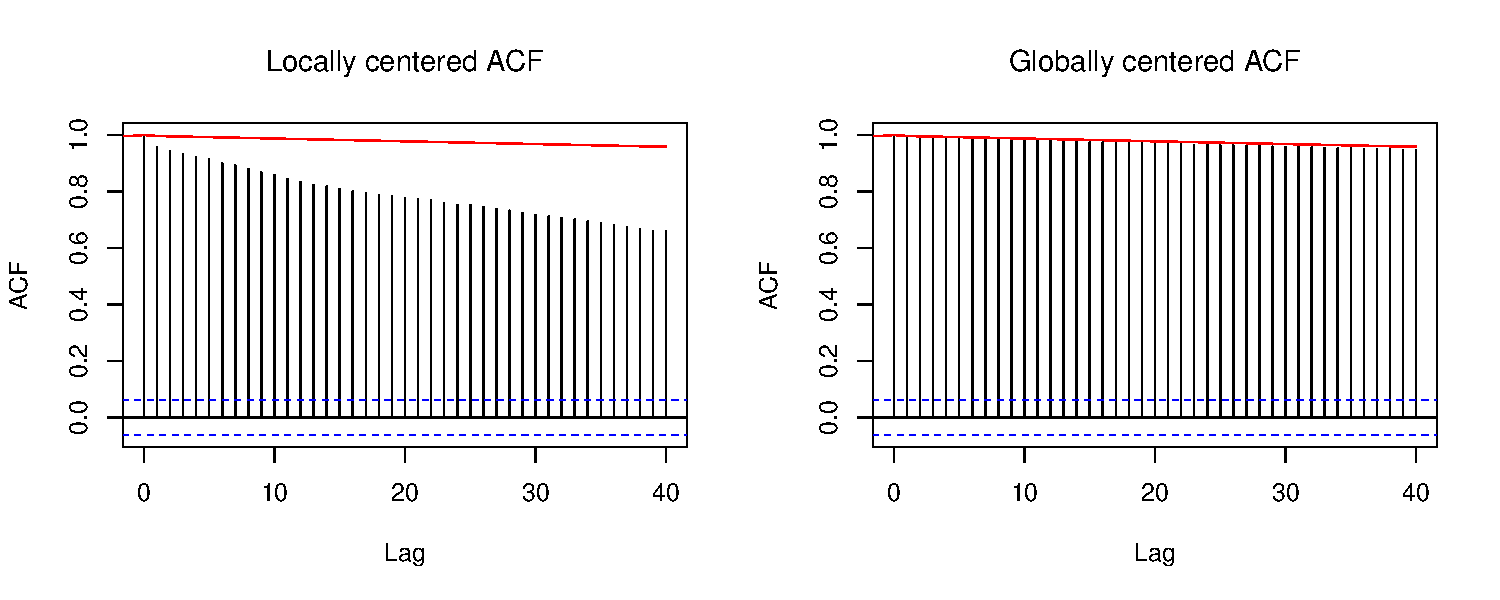
\includegraphics[width=.7\linewidth]{plots/var-acf_n1000.pdf}
   \caption{$n = 10^3$}
   \label{subfig:var-acf_n1e3}
\end{subfigure}\\
\begin{subfigure}[h]{\textwidth}
  \centering
  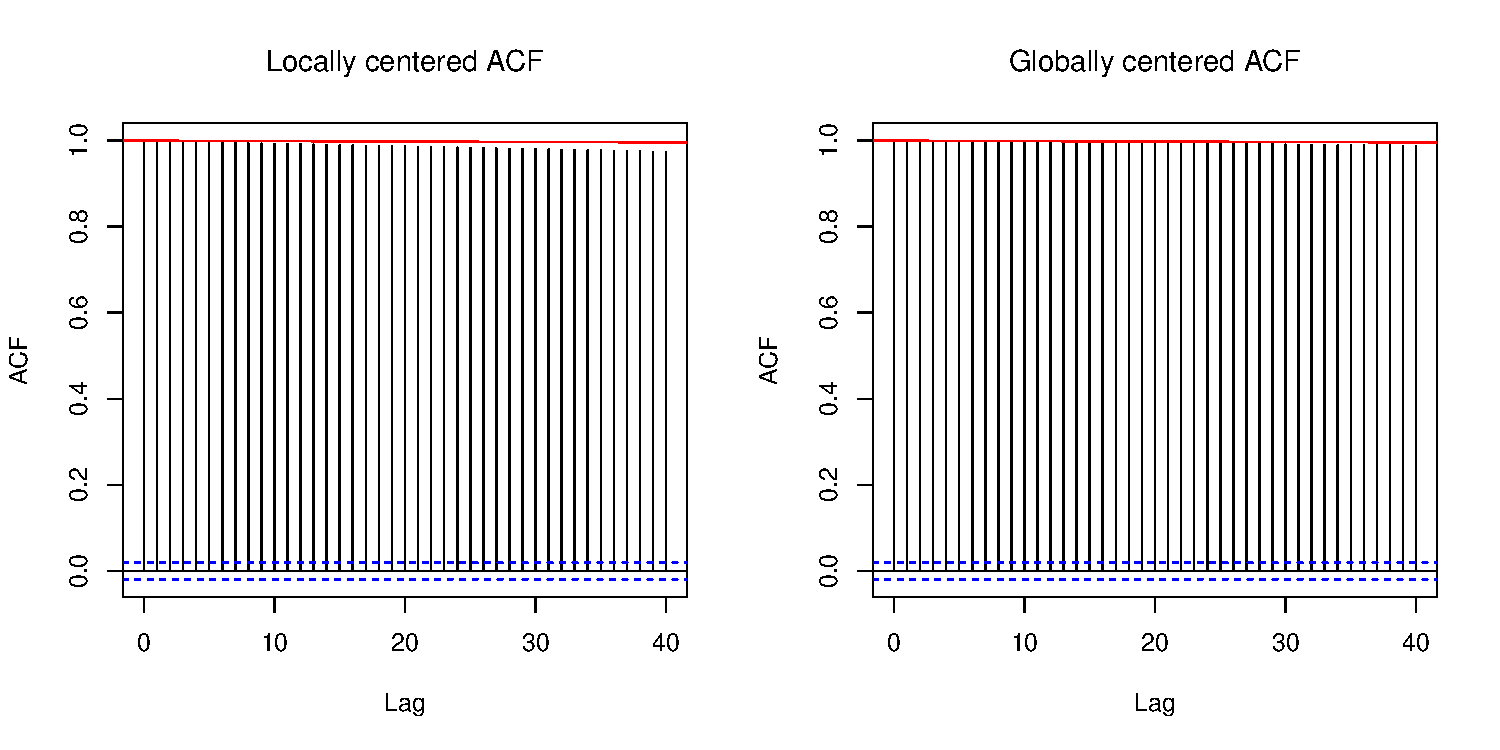
\includegraphics[width=.7\linewidth]{plots/var-acf_n10000.pdf} 
  \caption{$n = 10^4$}
  \label{subfig:var-acf_n1e4}
\end{subfigure}

\caption{VAR(1). ACF (left) and G-ACF (right) for the second chain for $m=5$. (a): $n = 10^3$, not converged yet; (b): $n =  10^4$, converged. The red line marks the true ACF.}
\label{fig:var-acf}
\end{figure}

The locally and globally-centered autocorrelations for the second chain have been shown in Figure~\ref{fig:var-acf} for two different simulation sizes where the true ACF is shown by the red line. When the individual chains have not explored well, the local sample means have not converged to $\mu$. As a consequence, the single chain empirical ACF estimator severely underestimate the truth. Due to sufficiently dispersed starting values, G-ACF is closer to reality. In subfigure~\ref{subfig:var-acf_n1e4}, the convergence property of sample means has kicked in for each chain. Therefore, both the estimators provide equivalent results. Note that G-ACF reveals the true nature of ACF for almost ten times lesser chain length $n$.\\


\begin{figure}[h]
    \centering
    \begin{subfigure}{0.4\textwidth}
      \centering
      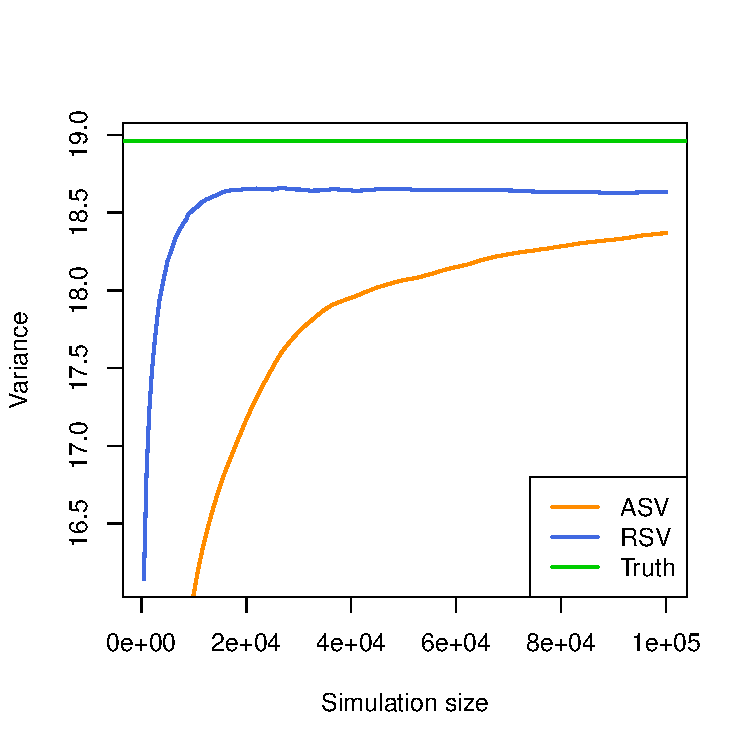
\includegraphics[width = \textwidth]{plots/var-frob.pdf}
      \caption{$log(\|\hat{\Sigma}\|_F)$}
      \label{subfig:var-frob}
    \end{subfigure}
    \begin{subfigure}{0.4\textwidth}
      \centering
      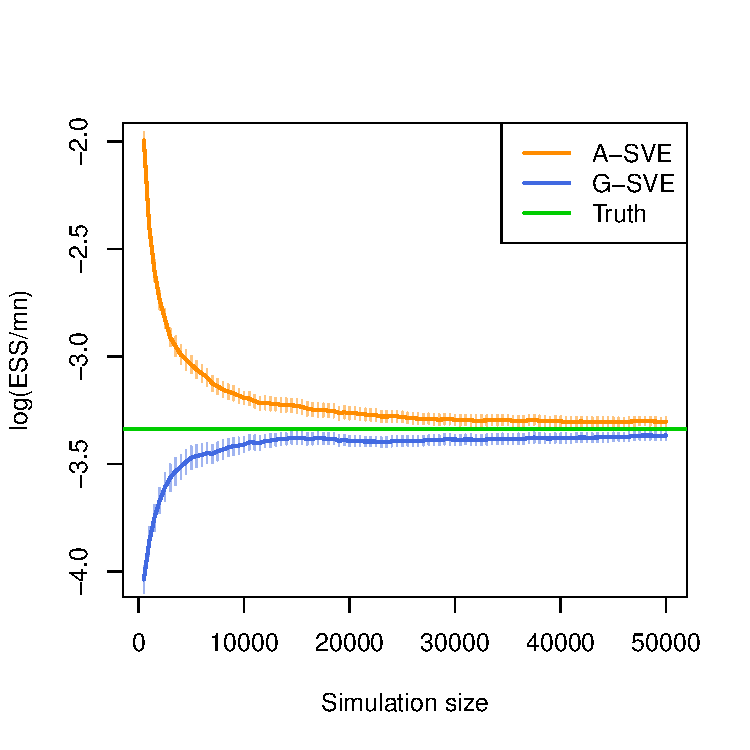
\includegraphics[width = \textwidth]{plots/var-ess.pdf}
      \caption{$\log(\widehat{\textrm{ESS}}/mn)$}
      \label{subfig:var-ess}
    \end{subfigure}
    \caption{VAR(1). (a) Running plot for logarithm of Frobenius norm of A-SVE and G-SVE from $n = 500$ to $n = 10^5$. (b) Running plot for logarithm of $\widehat{\textrm{ESS}}/mn$ calculated using A-SVE and G-SVE from $n=500$ to $n=10^5$.}
    \label{fig:var-frob_n_ess}
\end{figure}

The quality of estimation of $\Sigma$ and $\text{ESS}/mn$ has been studied through convergence of - (a) $\log(\|\hat{\Sigma}_A\|_F)$ and $\log(\|\hat{\Sigma}_G\|_F)$ as $n$ increases and (b) $\log(\widehat{\textrm{ESS}}_A/mn)$ and $\log(\widehat{\textrm{ESS}}_G/mn)$ as $n$ increases. In practice, it is preferred to slightly overestimate the variance and underestimate the ESS than do otherwise. In Figure~\ref{fig:var-frob_n_ess}, both the running plots are shown along with the green horizontal line which marks the truth. We run the simulations for 50 replications for each value of $n$ and plot the average as well as standard errors. We run the simulations for a maximum chain length of $5 \times 10^4$ when the estimators seem to have almost converged. From Figure~\ref{subfig:var-frob}, it can be seen that for first $10000$ samples, A-SV estimates can be absurdly small giving false confidence in single chain estimates whereas G-SV gives a better understanding of reality. Similar comparative argument can can given for ESS.


\begin{table}[h]
    \centering
    \begin{tabular}{|c|c|c|}
    \hline
    n & A-SVE & G-SVE\\
    \hline
    1000 & 0.71 & 0.956\\
    5000 & 0.843 & 0.937\\
    10,000 & 0.885 & 0.924\\
    50,000 & 0.928 & 0.945\\
    100,000 & 0.944 & 0.952\\
    \hline
    \end{tabular}
    \caption{VAR(1). Coverage probabilities for a $95$ percent confidence interval of global mean constructed using A-SVE and G-SVE as variance estimates around the known mean.}
    \label{tab:var-coverage}
\end{table}


We also report the coverage probabilities for a $95\%$ confidence interval constructed using $\hat{\Sigma}_A$ and $\hat{\Sigma}_G$ because the true mean is known here. Table~\ref{tab:var-coverage} shows that for each sample size, the globally-centered SV estimator for variance gives better coverage than A-SVE. At $n=10^5$, both the estimators have converged and give equivalently good coverage probability.


\subsection{Boomerang Distribution} \label{ex:boomerang}


Our globally-centered estimators perform exceptionally better than the single-chain estimators in case of multimodal target distribution. To that end, we will use a bivariate bi-modal distribution introduced by \cite{gelman1991note} which has Gaussian conditional distributions in both directions. This allows us to sample parallel Markov chains using the Gibbs sampler. Let $x$ and $y$ be two random variable that are jointly distributed as 
%
\[
f(x, y) \propto \exp\left(-\dfrac{1}{2} \left[Ax^2y^2 + x^2 + y^2 -2Bxy  -2C_1x - 2C_2y  \right]\right)
\]

The conditional distribution of $x$ given $y$ and vice versa is a normal distribution given by:
%
\begin{align*}
    x_1 \mid x_2 &\sim N\left(\dfrac{Bx_2 + C_1}{Ax_2^2 + 1}, \dfrac{1}{Ax_2^2 + 1}\right)\\
    x_2 \mid x_1 &\sim N\left(\dfrac{Bx_1 + C_2}{Ax_1^2 + 1}, \dfrac{1}{Ax_1^2 + 1}\right)
\end{align*}


\begin{figure}[h]
    \centering
    \begin{subfigure}[h]{.45\textwidth}
        \centering
        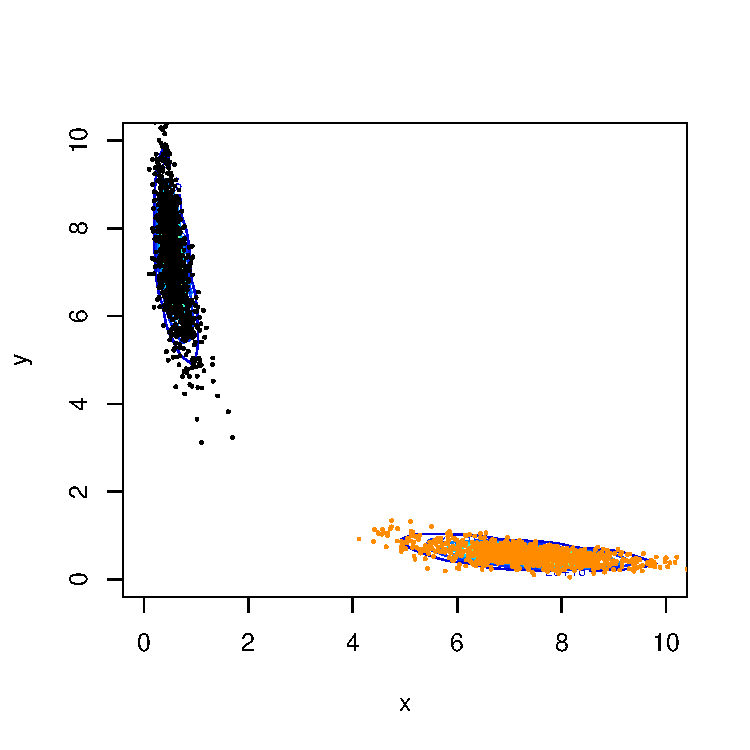
\includegraphics[width = \textwidth]{plots/boom-2d_density_plot_1_3_8.pdf}
        \caption{Setting-1}
        \label{subfig:boom-2D_1_3_8}
    \end{subfigure}
    \begin{subfigure}[h]{.45\textwidth}
        \centering
        \includegraphics[width = \textwidth]{plots/boom-2d_density_plot_1_10_7.pdf}
        \caption{Setting-2}
        \label{subfig:boom-2D_1_10_7}
    \end{subfigure}
    \caption{Boomerang. Contour plots of the target distribution for both settings. Overlayed scatter plot for two chains (in different colors) starting near each mode.}
   \label{fig:boom-2D}
\end{figure}


We report results for two different bi-modal parameter settings in this example. Firstly, we use a carefully chosen parameterization of $A = 1,\; B = 3,\; C = 8$ wherein the two modes are well-separated with a very low connection (Setting-1, Figure~\ref{subfig:boom-2D_1_3_8}). Secondly, to examine the performance of G-SVE for a nicely mixing Markov chain, we use the parametrization of $A = 1, \; B = 10, \; C=7$ wherein the two modes are closer and well-connected (Setting-2, Figure~\ref{subfig:boom-2D_1_10_7}). We will make another point through this example. For a fast mixing Markov chain, the globally-centered and locally-centered estimators give equivalent results. Therefore, it is a better practice to globally center the chains in any situation. We sample five parallel deterministically initialized chains with starting points dispersed uniformly in the first quadrant. Finding the actual mean of this distribution in closed form is difficult. Therefore, we use numerical integration with fine tuning to calculate it.

 To visualize the sticky nature of Markov chains in Setting-1, we show a scatter plot of two Markov chains starting near the two modes for $n = 1000$ in Figure~\ref{fig:boom-2D}. For the first thousand samples, both the chains are oblivious of the existence of another mode in setting-1. Whereas in setting-2, the chains have mixed fairly well for just $n=1000$.
 
 
\begin{figure}[h]
    \centering
    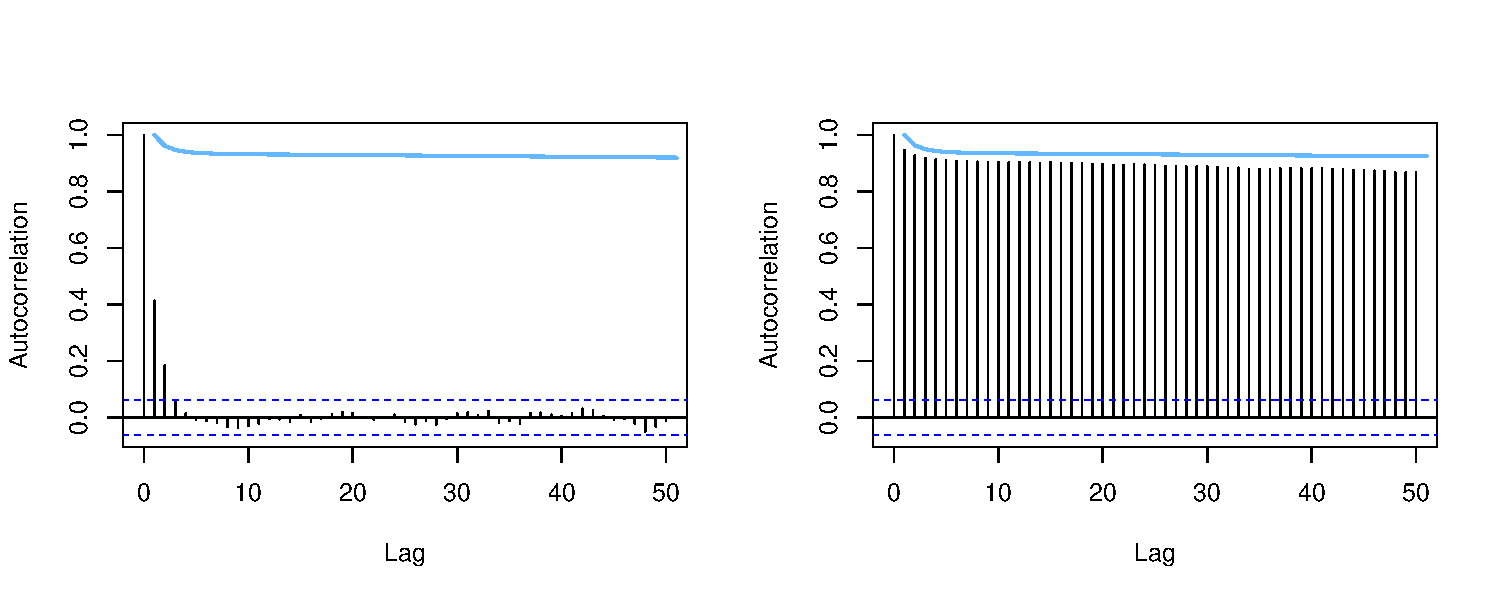
\includegraphics[width = .9\textwidth]{plots/boom-acf_1_3_8.pdf}
    \caption{Boomerang (setting-I). A-ACF (left) and G-ACF (right) of component-1 for $n=1000$ (histogram) and $n=10000$ (blue line) }
    \label{fig:boom-acf_1_3_8}
\end{figure}

\begin{figure}[h]
    \centering
    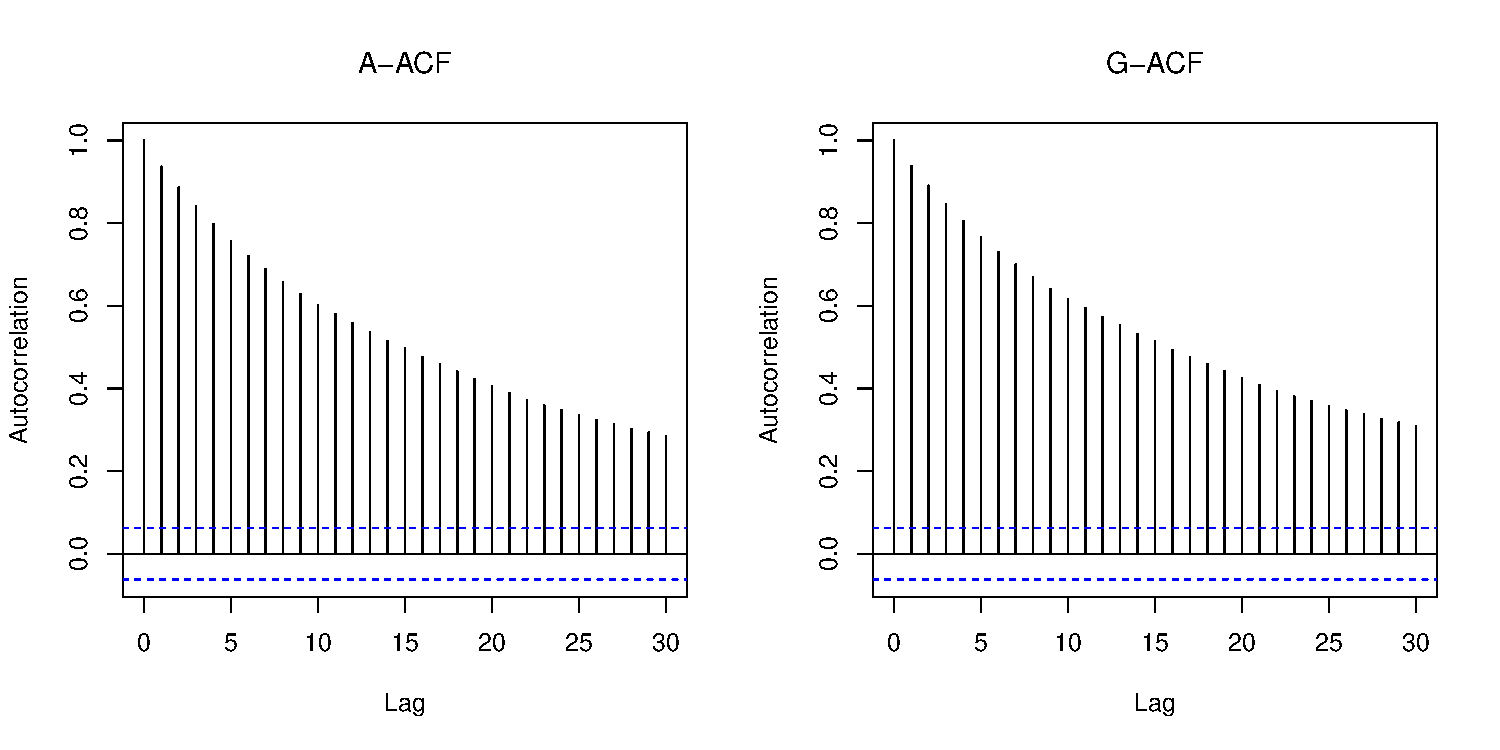
\includegraphics[width = 0.9\textwidth ]{plots/boom-acf_1_10_7_n1000.pdf}
    \caption{Boomerang. A-ACF (left) and G-ACF (right) of component-1 for $n=1000$}
    \label{fig:boom-acf_1_10_7}
\end{figure}

 
 In Figure \ref{fig:boom-acf_1_3_8}, the autocorrelations are severely underestimated by A-ACF for $n=1000$ because the chains have not jumped modes. Whereas, for $n=10000$, both ACF and G-ACF give almost indistinguishable results indicating that A-ACF and G-ACF have converged to the truth. We can observe in Figure~\ref{fig:boom-acf_1_10_7} that A-ACF and G-ACF give similar results for just $n=1000$ under simulation setting-2.


\begin{figure}[h]
    \centering
    
    \begin{subfigure}[h]{.4\textwidth}
      \centering
      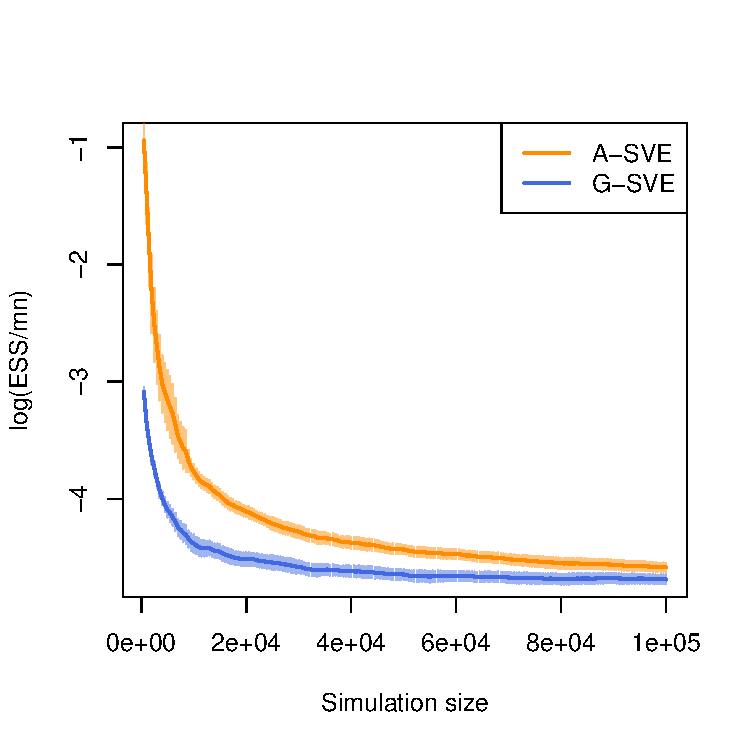
\includegraphics[width = \textwidth]{plots/boom-ess_1_3_8_m5.pdf}
      \caption{Setting-1}
      \label{subfig:boom-ess1}
    \end{subfigure} \hspace{1cm}
    \begin{subfigure}[h]{.4\textwidth}
      \centering
      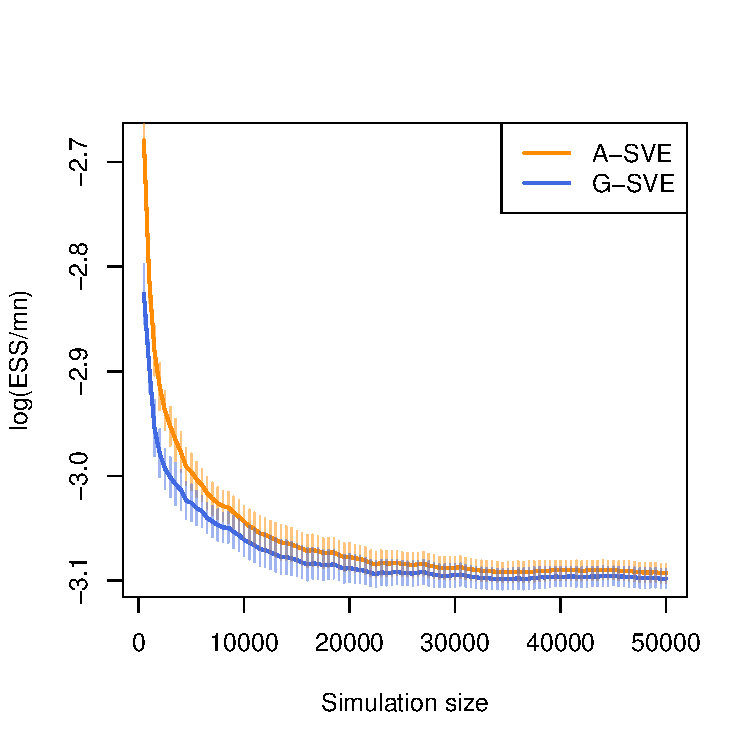
\includegraphics[width = \textwidth]{plots/boom-ess_1_10_7_m5.pdf}
      \caption{Setting-2}
      \label{subfig:boom-ess2}
    \end{subfigure}
    \caption{Boomerang. Running plot for $\log \hat{\text{ESS}}_A/mn$ and $\log \hat{\text{ESS}}_G/mn$ for $m = 5$.}
    \label{fig:boom-ess}
\end{figure}



\begin{figure}[h]
    \centering
    
    \begin{subfigure}[h]{.4\textwidth}
      \centering
      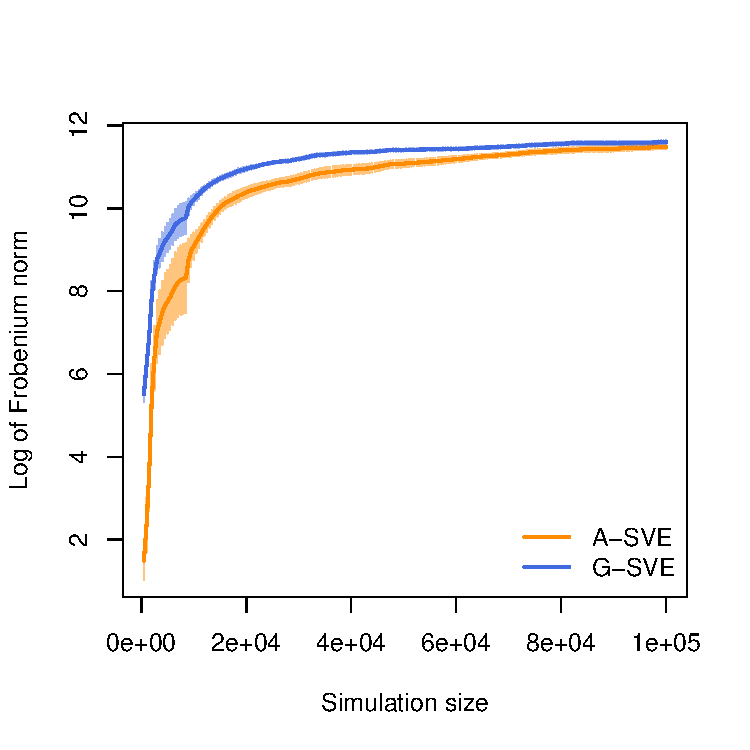
\includegraphics[width = \textwidth]{plots/boom-frob_1_3_8_m5.pdf}
      \caption{Setting-1}
      \label{subfig:boom-frob1}
    \end{subfigure} \hspace{1cm}
    \begin{subfigure}[h]{.4\textwidth}
      \centering
      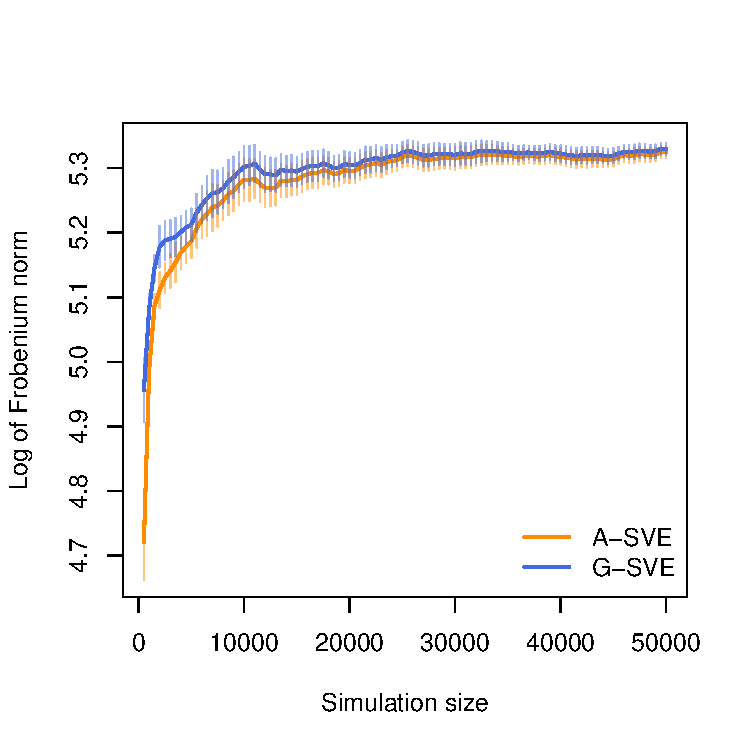
\includegraphics[width = \textwidth]{plots/boom-frob_1_10_7_m5.pdf}
      \caption{Setting-2}
      \label{subfig:boom-frob2}
    \end{subfigure}
    \caption{Boomerang. Running plot for $\log \|\hat{\Sigma}_A\|_F$ and $\log \|\hat{\Sigma}_G\|_F$ for $m = 5$.}
    \label{fig:boom-frob}
\end{figure}

The convergence of $\log \widehat{\textrm{ESS}}_G/mn$ and $\log \widehat{\textrm{ESS}}_A/mn$ as $n$ increases can be seen in Figure~\ref{fig:boom-ess}. We can see that in the beginning, A-SVE gives misleadingly higher estimates of ESS$/mn$ than G-SVE. This can cause us to stop the sampling before each chain jumps to the other mode. As a consequence, each chain will correspond to a uni-modal target distribution. Whereas, as expected, the ESS estimates for setting-2 are almost same. Similarly, $\|\hat{\Sigma}_G\|_F$ reaches the convergence point in less than half the time as $\|\hat{\Sigma}_G\|_F$; as evidenced in Figure~\ref{subfig:boom-frob1}. No significant difference can be observed for setting-2 (Figure~\ref{subfig:boom-frob2}).

\begin{table}[h]
\parbox{.45\linewidth}{
\centering
\begin{tabular}{|c|c|c|c|c|}
\hline
 $n$ & \multicolumn{2}{|c|}{$m = 2$} & \multicolumn{2}{|c|}{$m=5$}\\
 \hline
 & A-SVE & G-SVE & A-SVE & G-SVE \\
 \hline
 5000 & 0.595 &  0.7 & 0.402 &  0.64\\
 10000 & 0.563 &  0.665 & 0.59 &  0.739\\
 50000 & 0.775 &  0.814 & 0.807 &  0.864\\
 100000 & 0.847 &  0.864 & 0.884 &  0.902\\
\hline
\end{tabular}
\caption{Setting-1}
\label{tab:boom-coverage_1}
}
\hfill
\parbox{.45\linewidth}{
\centering
\begin{tabular}{|c|c|c|c|c|}
 \hline
 $n$ & \multicolumn{2}{|c|}{$m = 2$} & \multicolumn{2}{|c|}{$m=5$}\\
 \hline
 & A-SVE & G-SVE & A-SVE & G-SVE \\
 \hline
 1000 &  0.856 &  0.868 & 0.895 &  0.9100\\
 5000 & 0.921 &  0.925 & 0.91 &  0.915\\
 10000 & 0.928 &  0.93 & 0.919 &  0.926\\
 50000 & 0.943 &  0.944 & 0.951 &  0.952\\
\hline
\end{tabular}
\caption{Setting-2}
\label{tab:boom-coverage_2}
}
\end{table}

Using the numerical approximation of the true mean, we construct the $95\%$ confidence interval using A-SVE and G-SVE. We report the coverage probabilities for a 1000 replications at different sample sizes $n$. For both the simulation settings, we provide coverage probabilities for $m=2$ and $m=5$. Table \ref{tab:boom-coverage_1}, \ref{tab:boom-coverage_2} reports all these results. In setting-1, it can be observed that G-SVE gives higher coverage probability than A-SVE for all values of $n$. Whereas for setting-2, the results are almost similar indicating the equivalence of A-SVE and G-SVE.



\subsection{Sensor Network Localization}

For our third example, we consider a real-life example of sensor locations previously discussed by \cite{ihler2005nonparametric}. The goal is to identify unknown sensor locations using noisy distance data. This problem is specifically interesting in our case because the marginal posterior distribution for missing sensor locations is multi-modal for all locations. 

Following \cite{tak2018repelling}, we assume that there are six sensors scattered on a planar region where $x_i = (x_{i1}, x_{i2})^T$ denote the $2d$ coordinates of $i^{th}$ sensor. Let $y_{ij} = (y_{ji})$ denote the distance between the sensors $x_i$ and $x_j$. The distance between $x_i$ and $x_j$ is observed with probability $\pi (x_i, x_j) = \exp{\|x_i - x_j\|^2 / 2R^2}$ and with a Gaussian measurement error of $\sigma^2$. Let $z_{ij}$ denote the indicator variable which is equal to 1 when the distance between $x_i$ and $x_j$ is observed. The probability model is then,
%
\begin{align*}
    z_{ij} \mid x_1, ..., x_6 & \sim \text{Bernoulli}\left(\exp\left(\dfrac{-\|x_i - x_j\|^2}{2R^2}\right)\right)\\
    y_{ij} \mid w_{ij} = 1, x_1, ..., x_6 &\sim N(\|x_i - x_j\|^2, \sigma^2)
\end{align*}
%
\cite{ahn2013distributed} suggested the value of $R = 0.3$ and $\sigma = 0.02$. We use a Gaussian prior for the unknown locations with  mean equal to $(0,0)$ and covariance matrix equal to $100 I_2$. $y_{ij}$ is specified only if $w_{ij} = 1$. We follow the Markov chain structure as described by \cite{tak2018repelling} and sample from the four bivariate conditionals for each sensor location using a Gibbs sampler. In their paper on Repelling Attractive Metropolis (RAM) algorithms, \cite{tak2018repelling} compare the performance of different sampling techniques and show that RAM improves the acceptance rate by a factor of at least 5.5 over Metropolis using the same jumping scale. RAM algorithm supplies Markov chains with higher jumping frequency between the modes.

\begin{figure}[h]
    \centering
    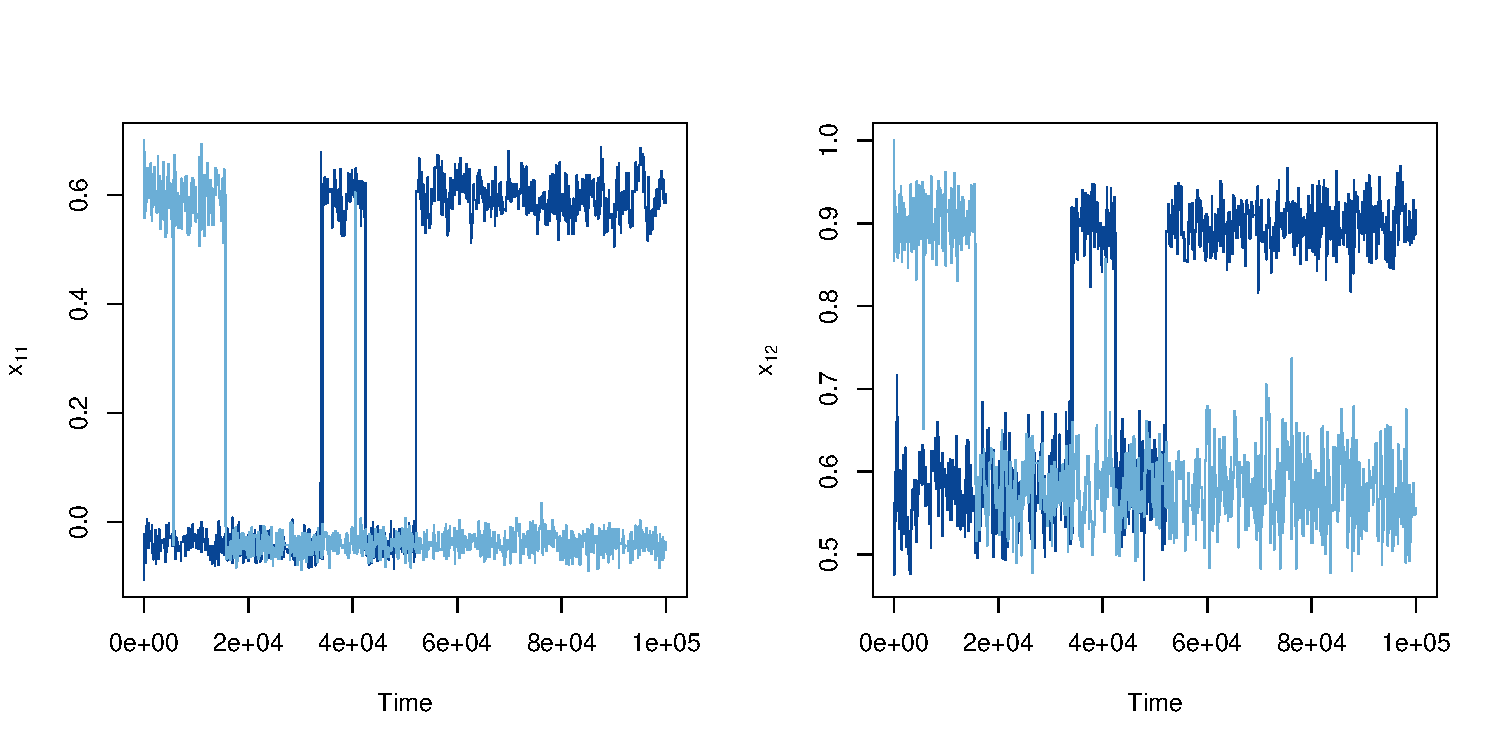
\includegraphics[width = .9\textwidth]{sensor-trace_loc1.pdf}
    \caption{Sensor Network. Trace plot of two chains for x (left) and y (right) coordinate of sensor location-1.}
    \label{fig:sensor-trace}
\end{figure}

This is an 8-dimensional estimation problem where the components corresponds to x and y coordinates of four unknown sensor locations. We will use the RAM algorithm with a jumping scale equal to $0.5$ to sample five parallel Markov chains with well-separated starting points. The total simulation size for each chain is fixed at $100,000$. Since the truth about actual mean and asymptotic variance is not known in this case, we are not interested in coverage probabilities.\\

To illustrate the \textit{sticky} nature of the Markov chains, we plot the evolution of two chains (starting near different modes) with time. Figure~\ref{fig:sensor-trace} shows the trace plot of x and y coordinate of sensor location-1. It is evident that the marginal posterior for both the components is bimodal. Similarly, the other three locations also have a bimodal marginal distribution in each component.  Observe that each chain explores one particular mode for a long time before jumping to another mode. \\

\begin{figure}[h]
    \centering
    \begin{subfigure}[h]{.45\textwidth}
      \centering
      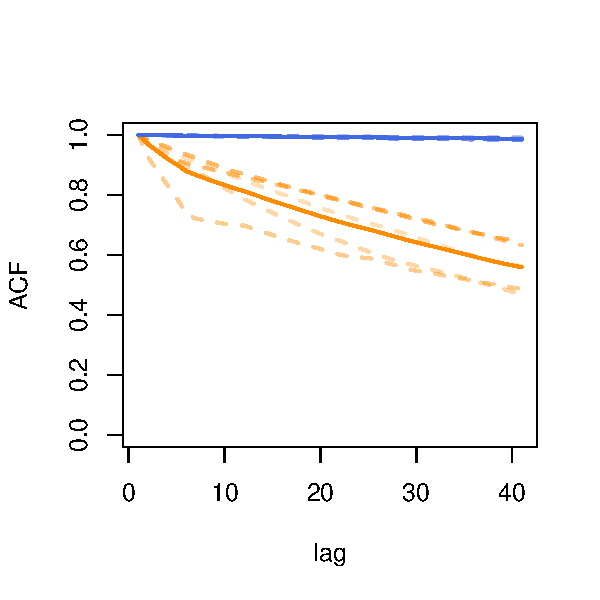
\includegraphics[width = \textwidth]{plots/sensor-acf_n5e3.pdf}
      \caption{$n = 5 \times 10^3$}
      \label{subfig:sensor-acf_5e3}
    \end{subfigure}
    \begin{subfigure}[h]{.45\textwidth}
      \centering
      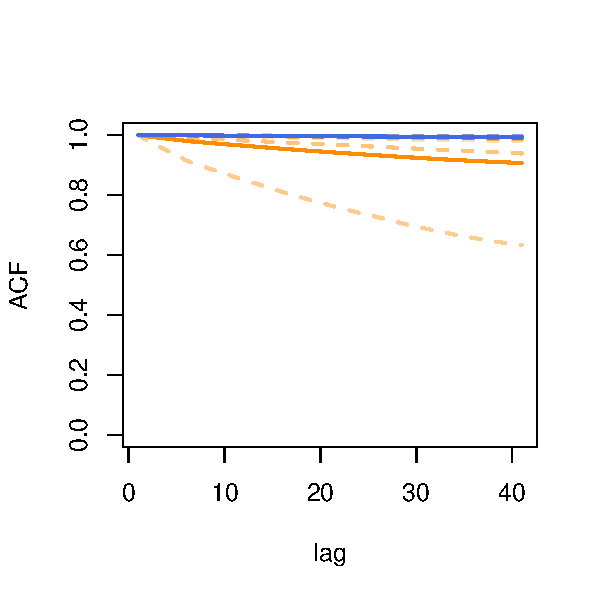
\includegraphics[width = \textwidth]{plots/sensor-acf_n5e4.pdf}
      \caption{$n = 5 \times 10^4$}
      \label{subfig:sensor-acf_5e4}
    \end{subfigure}
    \caption{Sensor Network. ACrF (orange) and G-ACrF (blue) for individual chains (dotted lines) and average over all chains (thick solid line).}
    \label{fig:sensor-acf}
\end{figure}

\begin{figure}
    \centering
    \begin{subfigure}[h]{0.4\textwidth}
      \centering
      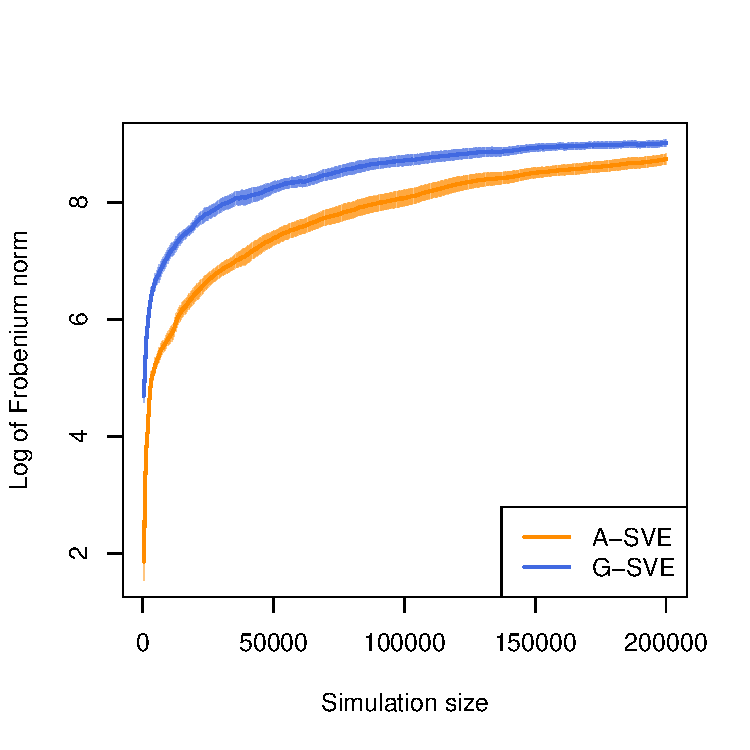
\includegraphics[width = \textwidth]{plots/sensor-frob.pdf}
      \caption{log Frobenius norm}
      \label{subfig:sensor-frob}
    \end{subfigure}
    \begin{subfigure}[h]{0.4\textwidth}
      \centering
      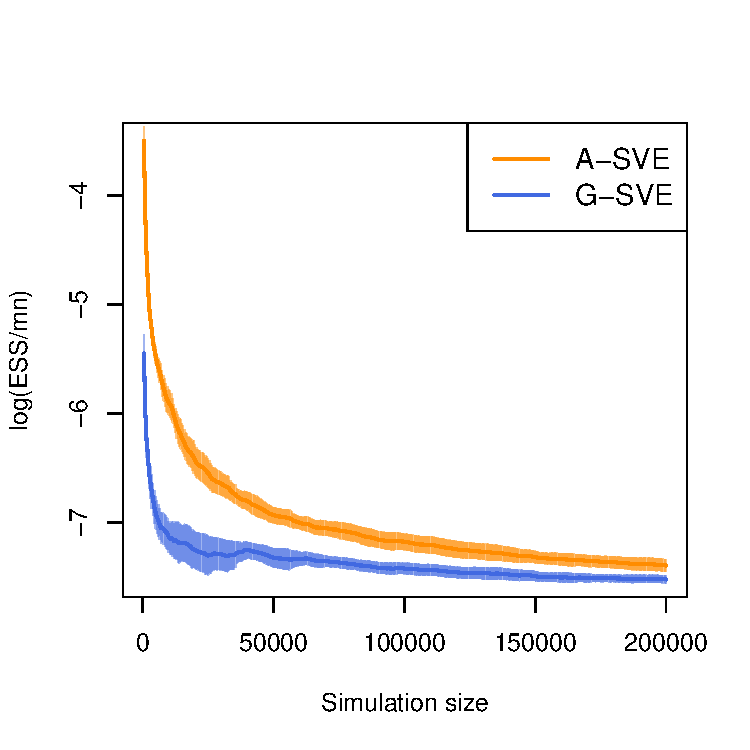
\includegraphics[width = \textwidth]{plots/sensor-ess.pdf}
      \caption{$\log(\widehat{\textrm{ESS}}/mn)$}
      \label{subfig:sensor-ess}
    \end{subfigure}
    \caption{Sensor Network. Running plot for $\log \|{\Sigma}\|_F$ (left) and $\log {\textrm{ESS}}/mn$ (right) estimated using A-SVE and G-SVE along with standard errors for 10 replications.}
    \label{fig:sensor-frob_n_ess}
\end{figure}

Figure~\ref{fig:sensor-acf} plots the locally and globally centered ACF estimators for individual chains  as well as the average over all the chains. The thick solid line plots the averaged estimator and the thin dotted lines correspond to ACF calculated using single chains. Figure~\ref{fig:sensor-frob_n_ess} presents the running plot of $\log \|{\Sigma}\|_F$ and $\log \textrm{ESS}/mn$ estimated using A-SVE and G-SVE along with standard errors from $10$ replications for each value of $n$. In both the plots, G-SVE and $\widehat{\textrm{ESS}}_G/mn$ reach the convergence value faster.

 
\section{Discussion} \label{sec:discussion}


In case of slowly mixing Markov chains or multimodal target distributions, the traditional single chain empirical estimator for ACvF can excruciatingly underestimate the truth. This will have serious impact on estimation of lag covariances, large sample variance of Monte Carlo averages, and determining when to stop the simulation process. It has been concluded in the paper that all of this can be significantly avoided by sampling multiple chains starting from dispersed points and pooling in the information from all chains to build consistent estimators for $\Gamma(k)$, $\Sigma$, and ESS. We have derived the bias of G-ACvF. We have shown that not only G-ACvF is asymptotically unbiased but also counters the negative bias of single chain ACF estimator by an amount proportional to the number of chains $m$. We have also proved the strong consistency of G-SVE and derived its limiting bias and variance results. Although the asymptotic results for G-SVE match those for SVE in \cite{andr:1991}, finite sample advantages are observed in terms of better coverage probability and faster convergence to truth.  



% Calculation of exact ACF has been done for simple stationary stochastic models like autoregressive (AR) models (under assumption of stationarity), moving average (MA) (\cite{quenouille1947notes}), and autoregressive-moving-average (ARMA) (\cite{box2015time}) models. We have already shown the impact of G-ACF for VAR(1) model where the truth is known. This gives us sufficient reason to believe that similar advantage will be observed for all the other models mentioned above in case of slowly mixing chains. Comparison to truth will reveal similar behavior However, for most of the complex sampling algorithms (including MCMC), we rely on sample estimators for ACF. 

For the purpose of experimentation in Section~\ref{sec:examples}, Bartlett lag window has been used throughout. Lag window comparisons done by \cite{andr:1991} reveal that quadratic spectral (QS) lag window gives consistently better coverage probabilities for any confidence interval. However, SVE gives poor coverage probability for all lag windows when the amount of autocorrelation is high in the Markov chain. Recently, \textit{lugsail} lag window has been proposed by \cite{vats2018lugsail} to deal with this issue by deliberately accentuating the autocovariance at smaller lags. We have refrained from doing lag window comparisons for G-SVE in our examples but we believe it can help improve the estimation quality significantly.
%

Another class of estimators for asymptotic variance of Monte Carlo averages are the multivariate initial sequence (mIS) estimators \citep{dai:jon:2017}. Similar to SV estimator, lag-covariances form the fundamental part of mIS estimators. In case of multi-modal target distributions, single chain mIS estimator will suffer from the same drawbacks as SVE. In this paper, we have chiefly focused on the usage of G-ACvF for estimating autocovariances in SVE; however the argument for a similar usage in mIS is straightforward.  Following \cite{dai:jon:2017}, generalised variance estimates obtained from mIS consistently overestimate $\abs{\Sigma}$. From Theorem~\ref{th:G-ACF_bias}, one can prove that, on average, the eigenvalues of $\hat{\Gamma}_{G,s}(k)$ are greater than the eigenvalues of $\hat{\Gamma}_s(k)$. This supplies readers with sufficient motivation to believe that the generalized variance for mIS constructed from $\hat{\Gamma}_G(k)$ not only consistently overestimates $\abs{\Sigma}$ but also upper-bounds the mIS from empirical single chain estimator of $\Gamma(k)$ for finite samples. An valuable line of research would be to prove these observations and carry out the theoretical analysis of mIS estimators using G-ACvF. 
%

The choice of starting vector is crucial for multiple chain sampling. In case the chains are started very near to each other, all the chains will explore nearly the same neighborhood in the state space. As a consequence, the G-ACvF will be equivalent to A-ACvF, and no significant improvement will be observed in estimation quality. We have used a deterministic initialization method in our examples using our prior knowledge about the location of modes in the target distribution. Comparing existing initialization methods {\color{orange} MA: maybe cite a few} and developing new ones could be an interesting direction for future research.  

\section{Appendix}  \label{sec:appendix}
\subsection{Preliminaries} \label{apdx:preliminaries}

\begin{lemma}
\label{lemma: brownian}
(\cite{csorgo2014strong}). Suppose the conditions of Theorem~\ref{thm:kuelbs} hold, then for all $\epsilon > 0$ and for almost all sample paths, there exists $n_{0}\left(\epsilon\right)$ such that $\forall n\geq n_{0}$ and $\forall i = 1, ..., p$

\[
\sup_{0\leq t \leq n-b_n}\sup_{0 \leq s \leq b_n} \left| B^{\left(i\right)}\left(t+s\right) - B^{\left(i\right)}\left(t\right) \right| < \left(1+ \epsilon\right)\left(2b_n\left(\log\dfrac{n}{b_n} + \log\; \log\; n\right)\right)^{1/2} ,
\]
%
\[
\sup_{0 \leq s \leq b_n} \left|B^{\left(i\right)}\left(n\right) - B^{\left(i\right)}\left(n - s\right)\right| < \left(1+ \epsilon\right)\left(2b_n\left(\log\dfrac{n}{b_n} + \log\;\log\;n\right)\right)^{1/2} , \;and
\]
%
\[
\left|B^{\left(i\right)}\left(n\right)\right| < \left(1+\epsilon\right)\sqrt{2n\;\log \log n} \; . 
\]
\end{lemma}


% \begin{lemma} \label{lemma:consis_1}
%   If Assumption~\ref{ass:sip} holds, then $\| \bar{\bar{X}} - \mu\|_{\infty}, \|\bar{X}_s - \mu\|_{\infty} \xrightarrow[]{a.s.} 0$ as $n \to \infty$ for all $s \in \{1,..., m\}$\\
%   \end{lemma}

% \begin{proof}
% Let $\|.\|$ denote the Euclidean norm. Assumption \ref{ass:sip} allows us to upper bound $\|\bar{X}_s - \mu\|_{\infty}$ using SIP. Following that, we show that the upper bound term converges to 0 as $n \to \infty$ using lemma \ref{lemma: brownian}.
%  \begin{align*}
%     \|\bar{X}_s - \mu\|_{\infty} & \leq \|\bar{X}_s - \mu\| \\
%     &= \dfrac{1}{n}\left\|\sum_{t=1}^{n}X_{st} - n\mu\right\| = \dfrac{1}{n}  \left \|\sum_{t=1}^{n}X_{st} - n\mu \pm L B(n) \right\|\\
%     & \leq \dfrac{1}{n}\left\|\sum_{t=1}^{n}X_{st} - \mu - L B(n)\right\| + \dfrac{\left\|L B(n)\right\|}{n}\\
%     &< \dfrac{D\psi(n)}{n} + \dfrac{\|L B(n)\|}{n}\\
%     &< \dfrac{D\psi(n)}{n} + \dfrac{1}{n}\|L\| \left(\sum\limits_{i=1}^{p}|B^{(i)}(k)|^2\right)^{1/2}\\
%     & \leq \dfrac{D\psi(n)}{n} + \dfrac{1}{n}\|L\| p^{1/2}(1+\epsilon)\sqrt{2n \log\log n}\\
%     & \xrightarrow[]{a.s.} 0\;\; as \;\; n\to \infty
%  \end{align*}
% %
% Similarly one can easily show that $\|\bar{\bar{X}} - \mu\|_{\infty} \to 0$ as $n \to \infty$ using the same upper-bound as:
% % 
% \begin{align*}
%     \|\bar{\bar{X}} - \mu\|_{\infty} & \leq \|\bar{\bar{X}} - \mu\| = \dfrac{1}{m}\left \|\sum_{j=1}^{m}(\bar{X}_j- \mu) \right\| \leq \dfrac{1}{m}\sum_{j=1}^{m}\|\bar{X}_j - \mu\| \xrightarrow{a.s.} 0 \, \textrm{as } n \to \infty 
% \end{align*}
% \end{proof}


% \section{Proof of Theorems} \label{appendix:A}

\subsection{Proof of Theorem~\ref{th:G-ACF_bias}} 
\label{appendix:bias}

% \begin{proof}

 
We can break $\hat{\Gamma}_{G,s}$ into four parts for all $k \geq 1$ as:
%  \[
%  \hat{\Gamma}_{G} =  \dfrac{1}{m}\sum_{s=1}^{m}\hat{\Gamma}_s(k) - \dfrac{1}{mn}\sum_{s=1}^{m}\sum_{t=1}^{|k|}A_{st}^T - \dfrac{1}{mn}\sum_{s=1}^{m}\sum_{t=n-|k|+1}^{n}A_{st} + \dfrac{n-|k|}{mn}\sum_{s=1}^{m}(\bar{X}_s - \bar{\bar{X}})(\bar{X}_s - \bar{\bar{X}})^T\,,
%  \]
% %
% where $A_{st} = (X_{st}-\bar{X}_s)(\bar{X}_s - \bar{\bar{X}})^T$\\
% The expectation value of the first term is given by equation \ref{eq:priestly} and \ref{eq:song} while the other three terms contribute $o(1)$ terms.

 % \begin{proof}[Proof of Theorem~\ref{th:G-_expec}]
% \begin{lemma} \label{lemma:bias1}
% $\mathbb{E}\left[ \left(X_{11} - \bar{X}_1 \right) \left(\bar{X}_1 - \bar{\bar{X}} \right)^T \right] = \dfrac{m-1}{mn}\left(\sum\limits_{k=0}^{n-1}\Gamma(k) - \Sigma\right)$
% \end{lemma}
% \begin{proof}
% \begin{align*}
%     &\mathbb{E} \left[ \left(X_{11} - \bar{X}_1 \right) \left(\bar{X}_1 - \bar{\bar{X}} \right)^T \right]\\
%      &= \mathbb{E} \left[X_{11}\bar{X}_1^T \right] - \mathbb{E}\left[X_{11}\bar{\bar{X}}^T \right] + \mathbb{E} \left[\bar{X}_1\bar{\bar{X}}^T \right] - \mathbb{E} \left[\bar{X}_1\bar{X}_1^T \right]\\
%     &= \mathbb{E} \left[X_{11}\bar{X}_1^T \right] - \dfrac{1}{m}\mathbb{E} \left[X_{11}\bar{X}_1^T \right] - \dfrac{m-1}{m}\mathbb{E} \left[X_{11}\bar{X}_2^T \right] + \dfrac{1}{m}\mathbb{E} \left[\bar{X}_1\bar{X}_1^T \right] + \dfrac{m-1}{m}\mathbb{E} \left[\bar{X}_1\bar{X}_2^T \right] - \mathbb{E} \left[\bar{X}_1\bar{X}_1^T \right]\\
%     &= \dfrac{m-1}{m}\left(\mathbb{E} \left[X_{11}\bar{X}_1^T \right] - \mathbb{E} \left[X_{11}\bar{X}_2^T \right] + \mathbb{E} \left[\bar{X}_1\bar{X}_2^T \right] - \mathbb{E} \left[\bar{X}_1\bar{X}_1^T \right]\right)\\
%     &= \dfrac{m-1}{m}\left(\dfrac{1}{n}\sum_{t=1}^{n}\mathbb{E} \left[X_{11}X_{1t}^T \right] - \mathbb{E}\left[X_{11}\right] \mathbb{E}\left[\bar{X}_2^T \right] + \mathbb{E} \left[\bar{X}_1\right]\mathbb{E}\left[\bar{X}_2^T\right] - \text{Var}\left[\bar{X}_1 \right] - \mathbb{E}\left[\bar{X}_1 \right]\mathbb{E}\left[\bar{X}_1^T \right]\right)\\
%     &= \dfrac{m-1}{m}\left(\dfrac{1}{n}\sum_{k=0}^{n-1}\Gamma(k) + \mu \mu^T - \mu \mu^T + \mu \mu^T - \text{Var}\left[\bar{X}_1 \right] - \mu \mu^T\right)\\
%     &= \dfrac{m-1}{mn}\left(\sum_{k=0}^{n-1}\Gamma(k) - n\text{Var}\left[\bar{X}_1 \right]\right)\,.
% \end{align*}
% %
% Similarly,
% %    
% \begin{align*}
%     \mathbb{E} \left[ \left(\bar{X}_1 - \bar{\bar{X}} \right)  \left(X_{11} - \bar{X}_1 \right)^T \right] &= \mathbb{E}\left[ \left(X_{11} - \bar{X}_1 \right) \left(\bar{X}_1 - \bar{\bar{X}} \right)^T \right]^T = \dfrac{m-1}{mn}\left(\sum_{k=0}^{n-1}\Gamma(k) - \Sigma \right)^T\,.
%     % &= \dfrac{m-1}{mn}\left(\sum_{k=0}^{n-1}\Gamma(k) - \Sigma \right)\\
% \end{align*}
% \end{proof}


% \begin{lemma} \label{lemma:bias2}
% \[
% \mathbb{E}\left[\sum\limits_{s=1}^{m} \left(\bar{X}_{s} - \bar{\bar{X}} \right) \left(\bar{X}_{s} - \bar{\bar{X}} \right)^{T}\right] =  (m-1)\text{Var}(\bar{X}_1)\,.
% \]
% \end{lemma}

% % $\bar{X}_i$ are independently and identically distributed for all $i$; this implies $\Var(\bar{\bar{X}}) = \dfrac{1}{m} \Var(\bar{X}_1)$. 

% \begin{proof}
% \begin{align*}
% \mathbb{E}\left[\sum_{s=1}^{m} \left(\bar{X}_{s} - \bar{\bar{X}} \right)  \left(\bar{X}_{s} - \bar{\bar{X}} \right)^{T}\right] &= \mathbb{E}\left[\sum_{s=1}^{m}\bar{X}_{s}\bar{X}_{s}^{T} -\sum_{s=1}^{m}\bar{X}_{s}\bar{\bar{X}}^{T} - \bar{\bar{X}}^{T}\sum_{s=1}^{m}\bar{X}_{s}^{T} + m\bar{\bar{X}}\bar{\bar{X}}^{T}\right]\\
% &= \mathbb{E}\left[\sum_{s=1}^{m}\bar{X}_{s}\bar{X}_{s}^{T} - m\bar{\bar{X}}\bar{\bar{X}}^{T}\right]\\
% &= m\left(\mathbb{E}\left[\bar{X}_{1}\bar{X}_{1}^{T}\right] - \mathbb{E}\left[\bar{\bar{X}}\bar{\bar{X}}^{T}\right]\right)\\
% &= m\left(\Var(\bar{X}_{1}) + \mu\mu^{T} - \Var(\bar{\bar{X}}) - \mu\mu^{T}\right)\\
% &= (m-1)\Var(\bar{X_1})\,.
% \end{align*}
% \end{proof}



\begin{align*}
\hat{\Gamma}_{G,s}(k) & = \dfrac{1}{n}\sum_{t=1}^{n-|k|} \left(X_{st} - \bar{\bar{X}} \right) \left(X_{s(t+k)} - \bar{\bar{X}} \right)^T \\
    &= \left[\dfrac{1}{n} \sum_{t=1}^{n-|k|} \left(X_{st} - \bar{X}_s \right) \left(X_{s(t+k)} - \bar{X}_s \right)^T \right] + \left[\dfrac{1}{n} \sum_{t=1}^{|k|} \left(\bar{X}_s - \bar{\bar{X}} \right)  \left(\bar{X}_s - X_{st} \right)^T\right] \\ 
    & \quad +  \left[\dfrac{1}{n} \sum_{t=n-|k|+1}^{n}  \left( \bar{X}_s - X_{st} \right)  \left(\bar{X}_s - \bar{\bar{X}} \right)^T\right] + \left[\dfrac{n-|k|}{n} \left(\bar{X}_s - \bar{\bar{X}}\right)   \left(\bar{X}_s - \bar{\bar{X}} \right)^T\right]\\
    &= \hat{\Gamma}_s(k) - \dfrac{1}{n} \sum_{t=1}^{|k|}A_{st}^T - \dfrac{1}{n}\sum_{t=n-|k|+1}^{n}A_{st} + \dfrac{n-|k|}{n}  \left(\bar{X}_s - \bar{\bar{X}} \right)  \left(\bar{X}_s - \bar{\bar{X}} \right)^T\,, \numberthis \label{eq:acf_breakdown}
\end{align*}
%
where $A_{st} = (X_{st}-\bar{X}_s)(\bar{X}_s - \bar{\bar{X}})^T$. Under the assumption of stationarity, we will study the expectations of the each of the above terms. Without loss of generality, consider $A_{11}$,
\begin{align*}
    &\E \left[A_{11} \right]\\
     &= \mathbb{E} \left[ \left(X_{11} - \bar{X}_1 \right) \left(\bar{X}_1 - \bar{\bar{X}} \right)^T \right]\\
     % &= \mathbb{E} \left[X_{11}\bar{X}_1^T \right] - \mathbb{E}\left[X_{11}\bar{\bar{X}}^T \right] + \mathbb{E} \left[\bar{X}_1\bar{\bar{X}}^T \right] - \mathbb{E} \left[\bar{X}_1\bar{X}_1^T \right]\\
    &= \mathbb{E} \left[X_{11}\bar{X}_1^T \right] - \dfrac{1}{m}\mathbb{E} \left[X_{11}\bar{X}_1^T \right] - \dfrac{m-1}{m}\mathbb{E} \left[X_{11}\bar{X}_2^T \right] + \dfrac{1}{m}\mathbb{E} \left[\bar{X}_1\bar{X}_1^T \right] + \dfrac{m-1}{m}\mathbb{E} \left[\bar{X}_1\bar{X}_2^T \right] - \mathbb{E} \left[\bar{X}_1\bar{X}_1^T \right]\\
    &= \dfrac{m-1}{m}\left(\mathbb{E} \left[X_{11}\bar{X}_1^T \right] - \mathbb{E} \left[X_{11}\bar{X}_2^T \right] + \mathbb{E} \left[\bar{X}_1\bar{X}_2^T \right] - \mathbb{E} \left[\bar{X}_1\bar{X}_1^T \right]\right)\\
    &= \dfrac{m-1}{m}\left(\dfrac{1}{n}\sum_{t=1}^{n}\mathbb{E} \left[X_{11}X_{1t}^T \right] - \mathbb{E}\left[X_{11}\right] \mathbb{E}\left[\bar{X}_2^T \right] + \mathbb{E} \left[\bar{X}_1\right]\mathbb{E}\left[\bar{X}_2^T\right] - \text{Var}\left[\bar{X}_1 \right] - \mathbb{E}\left[\bar{X}_1 \right]\mathbb{E}\left[\bar{X}_1^T \right]\right)\\
    % &= \dfrac{m-1}{m}\left(\dfrac{1}{n}\sum_{k=0}^{n-1}\Gamma(k) + \mu \mu^T - \mu \mu^T + \mu \mu^T - \text{Var}\left[\bar{X}_1 \right] - \mu \mu^T\right)\\
    &= \dfrac{m-1}{mn}\left(\sum_{k=0}^{n-1}\Gamma(k) - n\text{Var}\left[\bar{X}_1 \right]\right)\,. \numberthis \label{eq:acf_2}
\end{align*}
%
Similarly,
%    
\begin{align}
\label{eq:acf_3}
    \mathbb{E} \left[ A_{11}^T \right] &= \mathbb{E}\left[ A_{11}\right]^T = \dfrac{m-1}{mn}\left(\sum_{k=0}^{n-1}\Gamma(k)^T - n\text{Var}\left[\bar{X}_1 \right] \right)\,.
    % &= \dfrac{m-1}{mn}\left(\sum_{k=0}^{n-1}\Gamma(k) - \Sigma \right)\\
\end{align}


Further,
\begin{align*}
\mathbb{E}\left[ \left(\bar{X}_{1} - \bar{\bar{X}} \right)  \left(\bar{X}_{1} - \bar{\bar{X}} \right)^{T}\right] &= \mathbb{E}\left[ \bar{X}_{1}\bar{X}_{1}^{T} - \bar{X}_{1}\bar{\bar{X}}^{T} - \bar{\bar{X}} \bar{X}_{1}^{T} + \bar{\bar{X}}\bar{\bar{X}}^{T}\right]\\
% &= \mathbb{E}\left[ \bar{X}_{1}\bar{X}_{1}^{T} - \bar{\bar{X}}\bar{\bar{X}}^{T}\right]\\
% &= \left(\mathbb{E}\left[\bar{X}_{1}\bar{X}_{1}^{T}\right] - \mathbb{E}\left[\bar{\bar{X}}\bar{\bar{X}}^{T}\right]\right)\\
&= \left(\Var(\bar{X}_{1}) + \mu\mu^{T} - \Var(\bar{\bar{X}}) - \mu\mu^{T}\right)\\
&= \dfrac{m-1}{m}\Var(\bar{X}_1)\,. \numberthis \label{eq:acf_4}
\end{align*}
%
Additionally, the locally-centered autocovariance exhibits the following expectation (from \cite{priestley1981spectral})
 \begin{equation} \label{eq:priestly}
     \mathbb{E}[\hat{\Gamma}(k)] = \left(1- \dfrac{\abs{k}}{n}\right)\left(\Gamma(k) - \Var{(\bar{X})}
 \right)\,.
 \end{equation}
%
As a consequence, if $\Var(\bar{X})$ is finite, then $\Var(\bar{X}) \to 0 \textrm{ as } n \to \infty$.
Using \eqref{eq:priestly}, \eqref{eq:acf_2}, \eqref{eq:acf_3}, and \eqref{eq:acf_4} in \eqref{eq:acf_breakdown},
\begin{align*}
    & \E \left[\hat{\Gamma}_{G,s}(k) \right] \\
    &= \mathbb{E}\left[\hat{\Gamma}_{s}(k)\right] - \dfrac{1}{n} \left(\sum\limits_{t=1}^{|k|}\mathbb{E}[A_{1t}^T] + \sum\limits_{t=n-|k|+1}^{n}\mathbb{E}[A_{1t}]\right) + \left(1- \dfrac{|k|}{n}\right)\left(1-\dfrac{1}{m}\right)\Var(\bar{X}_1)\\
    &= \mathbb{E}\left[\hat{\Gamma}_{s}(k)\right] - \dfrac{|k|}{n}\left(1-\dfrac{1}{m}\right)\left(\dfrac{1}{n}\sum_{h=0}^{n-1}\Gamma(h) + \dfrac{1}{n}\sum_{h=0}^{n-1}\Gamma(h)^T - 2 \Var(\bar{X}_1)\right) + \left(1- \dfrac{|k|}{n}\right)\left(1-\dfrac{1}{m}\right)\Var(\bar{X}_1)\\
    &= \left(1- \dfrac{|k|}{n}\right)\Gamma(k) - \dfrac{|k|}{n}\left[\left(1-\dfrac{1}{m}\right)\left(\dfrac{1}{n}\sum_{h=0}^{n-1}\Gamma(h)^T + \dfrac{1}{n}\sum_{h=0}^{n-1}\Gamma(h)\right) - \left(2-\dfrac{1}{m}\right) \Var(\bar{X}_1)\right] - \dfrac{\Var(\bar{X}_1)}{m}\,.
\end{align*}
%

 We can use the results of \cite{song1995optimal} to expand $\Var(\bar{X}_1)$. By proposition 1 in \cite{song1995optimal} 
\[
\Var(\bar{X}) = \dfrac{\Sigma}{n} + \dfrac{\Phi}{n^2} + o(n^{-2})
\]

As a consequence, if $\Var(\bar{X})$ is finite, then $\Var(\bar{X}) \to 0 \textrm{ as } n \to \infty$. Expectation of $\hat{\Gamma}_{G,s}(k)$ can then broken down as following,
 \begin{equation} \label{eq:G-ACF_expec_breakdown}
     \mathbb{E}\left[\hat{\Gamma}_{G,s}(k)\right] = \left(1- \dfrac{|k|}{n}\right)\Gamma(k) + O_1 + O_2\,.
 \end{equation}
%
where,
\begin{align*}
    O_1 &= -\dfrac{|k|}{n}\left[\left(1-\dfrac{1}{m}\right)\left(\dfrac{1}{n}\sum_{h=0}^{n-1}\Gamma(h)^T + \dfrac{1}{n}\sum_{h=0}^{n-1}\Gamma(h)\right) - \left(2-\dfrac{1}{m}\right) \left(\dfrac{\Sigma}{n} + \dfrac{\Phi}{n^2}\right)\right] + o(n^{-2})\, ,\\
    O_2 &= -\dfrac{1}{m}\left(\dfrac{\Sigma}{n} + \dfrac{\Phi}{n^2}\right) + o(n^{-2})
\end{align*}
%
We observe that both $O_1 \textrm{ and } O_2$ are small order terms that converge to 0 as $n \to \infty$. Here, $O_1 = (-\abs{k}/n)\mathcal{O}(1/n) \textrm{ and } O_2 = {\mathcal{O}}(1/n)$. For a diagonal element of $\Gamma$,
% We observe that this expectation result is very similar to equation \ref{eq:priestly} from \cite{priestley1981spectral} for the asymptotically unbiased estimator of autocovariance except for an additional positive bias term. This helps in countering the inherent negative bias in $\hat{\Gamma}(k)$ and give more informative estimates of autocovariance.  Although, bias term for a fixed $k$ is $o(1)$, it increases with $k$. We have explicitly written the end effect term arising from using the estimator $\bar{\bar{X}}$ for $\mu$. These are small order terms that vanish as $n \to \infty$.
%
\begin{align*}
& \E \left[ \hat{\Gamma}_{G,s}^{ii}\right]\\
& = \mathbb{E}\left[\hat{\Gamma}^{ii}_{s}(k)\right] - \dfrac{|k|}{n}\left[\left(1-\dfrac{1}{m}\right)\left(\dfrac{1}{n}\sum_{h=0}^{n-1} \left[\Gamma^{ii}(h)^T + \Gamma^{ii}(h) \right] \right) - \left(2-\dfrac{1}{m}\right) \Var(\bar{X}_1)^{ii}\right] - \dfrac{\Var(\bar{X}_1)^{ii}}{m}\,.
\end{align*}
In the presence of positive correlation, the leftover term is positive.


% \begin{proof}[Proof of corollary \ref{cor:lag0_expectation}]

% \begin{align*}
%     \hat{\Gamma}_{G-}(0) &= \dfrac{1}{m}\sum_{s=1}^{m}\hat{\Gamma}_{G-,s}(0) = \dfrac{1}{mn}\sum_{s=1}^{m}\sum_{t=1}^{n}  \left(X_{st} - \bar{\bar{X}}\right)  \left(X_{st} - \bar{\bar{X}}\right)^T\\
%     &= \left[\dfrac{1}{mn}\sum_{s=1}^{m}\sum_{t=1}^{n} \left(X_{st} - \bar{X}_s \right)  \left(X_{st} - \bar{X}_s \right)^T\right] + \left[\dfrac{1}{m}\sum_{s=1}^{m} \left(\bar{X}_s - \bar{\bar{X}} \right) \left(\bar{X}_s - \bar{\bar{X}} \right)^T\right]\\
%     &= \dfrac{1}{m}\sum_{s=1}^{m}\hat{\Gamma}_s(0)  + \dfrac{1}{m}\sum_{s=1}^{m} \left(\bar{X}_s - \bar{\bar{X}} \right)  \left(\bar{X}_s - \bar{\bar{X}} \right)^T\,.
% \end{align*}
% Using \eqref{eq:priestly} and \eqref{eq:acf_4} the expectation of $\hat{\Gamma}_{G-}(0)$ can be written as 
% %
% \begin{align*}
%     \mathbb{E} \left[\hat{\Gamma}_{G-}(0) \right] &= \E\left[\hat{\Gamma}_1(0) \right] + \left(1-\dfrac{1}{m}\right)\Var(\bar{X}_1) \\
%     & = \Gamma(k) - \dfrac{1}{m}\Var(\bar{X}_1)\,.
%     % &= \Gamma(0) - \dfrac{\Sigma}{mn} - \dfrac{\Phi}{mn^2} + o(n^{-2})
% \end{align*}

% \end{proof}


\subsection{Strong consistency argument} \label{appendix:strong_consis}


Consider pseudo autocovariance and spectral variance estimators for the $s$th chain, denoted by $\tilde{\Upsilon}_s(k)$ and $\tilde{\Sigma}_s$ that use data centered around the unobserved actual mean $\mu$:
\begin{align*}
    \tilde{\Upsilon}_s(k) &= \dfrac{1}{n}\sum_{t=1}^{n-|k|}(Y_{st}-\mu_g)(Y_{s(t+k)}-\mu_g)^T \\ 
    \tilde{\Sigma}_s &= \sum_{k=-b_n+1}^{b_n-1}w\left(\dfrac{k}{b_n}\right)\tilde{\Upsilon}_s(k) \,.
\end{align*}
%
The average pseudo spectral variance estimator is
\[
\tilde{\Sigma} = \dfrac{1}{m}\sum\limits_{s=1}^{m}\tilde{\Sigma}_s
\]

Further, let
\begin{align*}
  M_1 & = \dfrac{1}{m}\sum\limits_{s=1}^{m}\left\{\sum\limits_{k=-b_n+1}^{b_n-1}w\left(\dfrac{k}{b_n}\right)\sum\limits_{t=1}^{n-|k|}\dfrac{1}{n}\left[ \left(Y_{st}-\mu_g \right)_i   \left(\mu_g-\bar{\bar{Y}} \right)_j +    \left(\mu_g-\bar{\bar{Y}} \right)_i  \left(Y_{s(t+k)}-\mu_g \right)_j \right]\right\}\,, \\ 
  %
M_2 &= \left(\mu_g-\bar{\bar{Y}} \right)_i   \left(\mu_g-\bar{\bar{Y}} \right)_j\sum\limits_{k=-b_n+1}^{b_n-1}\left(1-\dfrac{|k|}{n}\right)w\left(\dfrac{k}{b_n}\right)\,.
\end{align*}


\begin{lemma} \label{lemma:G-SVE_breakdown}
For the G-SVE estimator, $\hat{\Sigma}_{G}^{ij} = \tilde{\Sigma}^{ij} + M_1 + M_2$ and 
\[
|M_1 + M_2| \leq D^2 g_1(n) + D g_2(n) + g_3(n)\,,
\]
where
\begin{align*}
    g_1(n) &= (4+C_1)\dfrac{b_n \psi^2(n)}{n^2} - 4\dfrac{\psi^2(n)}{n^2} \to 0\\
    g_2(n) &= 2\sqrt{2}\|L\|p^{1/2}(1+\epsilon)\left[(4+C_1)\dfrac{b_n\psi(n)\sqrt{n\log \log n}}{n^2} - 4\dfrac{\psi(n)\sqrt{n\log \log n}}{n^2}\right] \to 0\\
    g_3(n) &= \|L\|^2 p (1+\epsilon)^2\left[(4+C_1)\dfrac{b_n \log\log n}{n} - 4 \dfrac{\log \log n}{n}\right] \to 0\,.
\end{align*}
\end{lemma}

\begin{proof}
The proof follows from standard algebraic calculations and is presented here for completeness. Consider,
\begin{align*}
\hat{\Sigma}_{G}^{ij} &= \dfrac{1}{m}\sum_{s=1}^{m} \sum_{k=-b_n+1}^{b_n-1}w\left(\dfrac{k}{b_n}\right)\dfrac{1}{n}\sum_{t=1}^{n-|k|} \left(Y_{st}-\bar{\bar{Y}} \right)_i \left(Y_{s(t+k)}-\bar{\bar{Y}} \right)_j\\
% &= \dfrac{1}{m}\sum_{s=1}^{m}\sum_{k=-b_n+1}^{b_n-1}w\left(\dfrac{k}{b_n}\right)\dfrac{1}{n}\sum_{t=1}^{n-|k|} \left[  \left\{\left(X_{st}-\mu_g \right)_i + \left(\mu_g-\bar{\bar{X}} \right)_i \right \}  \left\{ \left(X_{s(t+k)}-\mu_g \right)_j + \left(\mu_g-\bar{\bar{X}} \right)_j \right \} \right]\\
&= \dfrac{1}{m}\sum_{s=1}^{m}\sum_{k=-b_n+1}^{b_n-1}w\left(\dfrac{k}{b_n}\right)\dfrac{1}{n}\sum_{t=1}^{n-|k|}  \left[ \left(Y_{st}-\mu_g \right)_i  \left(Y_{s(t+k)}-\mu_g \right)_j+  \left(Y_{st} - \mu_g \right)_i    \left(\mu_g - \bar{\bar{Y}} \right)_j \right. \\  
& \quad + \left. \left(\mu_g-\bar{\bar{Y}} \right)_i  \left(Y_{s(t+k)}-\mu_g \right)_j + \left(\mu_g-\bar{\bar{Y}} \right)_i  \left(\mu_g-\bar{\bar{Y}}  \right)_j  \right]\\
& = \tilde{\Sigma}^{ij} + \left[(\mu_g-\bar{\bar{Y}})_i(\mu_g-\bar{\bar{Y}})_j\sum_{k=-b_n+1}^{b_n-1}\left(1-\dfrac{|k|}{n}\right)w\left(\dfrac{k}{b_n}\right)\right] \\ 
& \quad  + \dfrac{1}{m}\sum_{s=1}^{m}\sum_{k=-b_n+1}^{b_n-1}  w\left(\dfrac{k}{b_n}\right)\sum_{t=1}^{n-|k|}  \left[\dfrac{1}{n} \left(Y_{st} - \mu_g \right)_i \left(\mu_g - \bar{\bar{Y}} \right)_j + \dfrac{1}{n} \left(\mu_g-\bar{\bar{Y}} \right)_i  \left(Y_{s(t+k)}-\mu_g \right)_j \right] \\ 
& = \tilde{\Sigma}^{ij} + M_1 + M_2\,.
\end{align*}

Consequently
\[
\left|\hat{\Sigma}_{G}^{ij} - \tilde{\Sigma}^{ij}  \right| = |M_1 + M_2| \leq |M_1| + |M_2|\,.
\]
%
We first present a result which will be useful to use later. For any Markov chain $s$, 
\begin{align*}
  \|\bar{Y}_s - \mu_g\|_{\infty} & \leq \|\bar{Y}_s - \mu_g\| = \dfrac{1}{mn}\left\|\sum_{t=1}^{n}Y_{st} - n\mu_g\right\| \\
  % &= \dfrac{1}{n}  \left \|\sum_{t=1}^{n}X_{st} - n\mu_g \pm L B(n) \right\|\\
  & \leq \dfrac{1}{n}\left\|\sum_{t=1}^{n}Y_{st} - n \mu_g - L B(n)\right\| + \dfrac{\left\|L B(n)\right\|}{n}\\
  &< \dfrac{D\psi(n)}{n} + \dfrac{\|L B(n)\|}{n}\\
  &< \dfrac{D\psi(n)}{n} + \dfrac{1}{n}\|L\| \left(\sum\limits_{i=1}^{p}|B^{(i)}(n)|^2\right)^{1/2}\\
  & \leq \dfrac{D\psi(n)}{n} + \dfrac{1}{n}\|L\| p^{1/2}(1+\epsilon)\sqrt{2n \log\log n}\,. \numberthis \label{eq:xbars_bound}
  % & \xrightarrow[]{a.s.} 0\;\; as \;\; n\to \infty 
\end{align*}
 %
 Similarly,
 \begin{equation}
\label{eq:xbarbar_bound}
   \| \bar{\bar{Y}} - \mu_g\|_{\infty} \leq \dfrac{D\psi(n)}{n} + \dfrac{1}{n}\|L\| p^{1/2}(1+\epsilon)\sqrt{2n \log\log n}\,.
\end{equation}
%  \begin{align*}
%   \| \bar{\bar{X}} - \mu_g\|_{\infty} & \leq \|\bar{\bar{X}} - \mu_g\| = \dfrac{1}{n}\left\|\sum_{s=1}^{m} \left(\sum_{t=1}^{n}X_{st} - n\mu_g \right)\right\| \\
%   &\leq \dfrac{1}{m}\sum_{s=1}^{m}\dfrac{1}{n}  \left \| \sum_{t=1}^{n}X_{st} - n\mu_g \pm L B(n) \right\|\\
%   & \leq \dfrac{1}{m} \sum_{s=1}^{m} \dfrac{1}{n}\left\| \sum_{t=1}^{n}X_{st} - n \mu_g - L B(n)\right\| + \dfrac{\left\|L B(n)\right\|}{n}\\
%   &< \dfrac{D\psi(n)}{n} + \dfrac{\|L B(n)\|}{n}\\
%   &< \dfrac{D\psi(n)}{n} + \dfrac{1}{n}\|L\| \left(\sum\limits_{i=1}^{p}|B^{(i)}(k)|^2\right)^{1/2}\\
%   & \leq \dfrac{D\psi(n)}{n} + \dfrac{1}{n}\|L\| p^{1/2}(1+\epsilon)\sqrt{2n \log\log n}\,. \numberthis \label{eq:xbarbar_bound}
%   % & \xrightarrow[]{a.s.} 0\;\; as \;\; n\to \infty 
% \end{align*}
%
Now consider,
\begin{align*}
& |M_1| \\ 
   % & = \left|\dfrac{1}{m}\sum _{s=1}^{m}\left\{\sum_{k=-b_n+1}^{b_n-1}w\left(\dfrac{k}{b_n}\right)\sum_{t=1}^{n-|k|} \dfrac{1}{n}\left[ \left(X_{st} - \mu_g \right)_i  \left(\mu_g-\bar{\bar{X}} \right)_j + \left(\mu_g-\bar{\bar{X}} \right)_i  \left(X_{s(t+k)} - \mu_g \right)_j\right]\right\}\right| \\
   % & \leq \dfrac{1}{m}\sum_{s=1}^{m}\left\{\sum_{k=-b_n+1}^{b_n-1}w\left(\dfrac{k}{b_n}\right)\left[ \dfrac{1}{n}{\left|\sum\limits_{t=1}^{n-|k|} \left(X_{st} - \mu_g \right)_i  \left(\mu_g - \bar{\bar{X}} \right)_j\right|} + \dfrac{1}{n}{\left|\sum_{t=1}^{n-|k|} \left(\mu_g-\bar{\bar{X}} \right)_i\left(X_{s(t+k)} - \mu_g \right)_j\right|} \right]\right\}\\
    & \leq \dfrac{1}{m}\sum_{s=1}^{m}\left\{\sum_{k=-b_n+1}^{b_n-1}w\left(\dfrac{k}{b_n}\right)\left[ \dfrac{1}{n}\left|\sum_{t=1}^{n-|k|}(Y_{st}- \mu_g)_i\right|\left|(\mu_g-\bar{\bar{Y}})_j\right|+ \dfrac{1}{n}\left|(\mu_g-\bar{\bar{Y}})_i\right|\left|\sum_{t=1}^{n-|k|}(Y_{j(t+k)}-\mu_g)_j\right|\right]\right\}\\
    & \leq \dfrac{\|(\bar{\bar{Y}} - \mu_g)\|_{\infty}}{m} \sum_{s=1}^{m}\sum\limits_{k=-b_n+1}^{b_n-1}\left[ \dfrac{1}{n}\left\|\sum_{t=1}^{n-|k|}(Y_{st}-\mu_g)\right\|_{\infty} + \dfrac{1}{n}\left\|\sum_{t=1}^{n-|k|}(Y_{s(t+k)}-\mu_g)\right\|_{\infty} \right]\\
    &\leq \dfrac{\|(\bar{\bar{Y}} - \mu_g)\|_{\infty}}{m} \\
    & \quad \times \sum_{s=1}^{m}\sum_{k=-b_n+1}^{b_n-1}\left[ \dfrac{1}{n}\left\|\sum_{t=n-|k|+1}^{n}(Y_{st} - \mu_g) - n(\bar{Y}_s - \mu_g) \right\|_{\infty} + \dfrac{1}{n}\left\|\sum_{t=1}^{|k|}(Y_{st} - \mu_g) - n(\bar{Y}_s - \mu_g)\right\|_{\infty} \right]\\
    &\leq \dfrac{\|(\bar{\bar{Y}} - \mu_g)\|_{\infty}}{m} \sum_{s=1}^{m}\sum\limits_{k=-b_n+1}^{b_n-1}\left[ \dfrac{1}{n}\left\|\sum_{t=n-|k|+1}^{n}(Y_{st} - \mu_g)\right\|_{\infty} + \dfrac{1}{n}\left\|\sum_{t=1}^{|k|}(Y_{st} - \mu_g)\right\|_{\infty} + 2\|\bar{Y}_s - \mu_g\|_{\infty} \right]\\
    & \leq \dfrac{\|(\bar{\bar{Y}} - \mu_g)\|_{\infty}}{m} \sum\limits_{s=1}^{m}\sum_{k=-b_n + 1}^{b_n-1}   \dfrac{1}{n}\left[\left\|\sum_{t=n-|k|+1}^{n}(Y_{st} - \mu_g)\right\|_{\infty} + \left\|\sum_{t=1}^{|k|}(Y_{st} - \mu_g)\right\|_{\infty} \right]\\
    & \; \;+ 2(2b_n - 1)\|\bar{\bar{Y}} - \mu_g\|_{\infty}\|\bar{Y}_1 - \mu_g\|_{\infty}\,.
\end{align*}
%
Using SIP on summation of $k$ terms, we obtain the following upper bound for $|M_1|$
\begin{align*}
|M_1|
    & < 2\|(\bar{\bar{Y}} - \mu_g)\|_{\infty} \left[\sum\limits_{k=-b_n + 1}^{b_n-1}\left[ \dfrac{D \psi(k)}{n} + \dfrac{\|L\| p^{1/2}(1+\epsilon)\sqrt{2k \log\log k}}{n}  \right] \right]  + 2(2b_n - 1) \|\bar{Y}_1 - \mu_g\|_{\infty} \\
    &\leq 2(2b_n - 1)\|(\bar{\bar{Y}} - \mu_g)\|_{\infty} \left[ \dfrac{D \psi(n)}{n} + \dfrac{\|L\| p^{1/2}(1+\epsilon)\sqrt{n \log\log n}}{n} + \|\bar{Y}_1 - \mu_g\|_{\infty}  \right]\\
    % & \quad  + 2(2b_n - 1)\|\bar{\bar{X}} - \mu_g\|_{\infty}\\
    & \leq 4(2b_n - 1)\left[ \dfrac{D \psi(n)}{n} + \dfrac{\|L\| p^{1/2}(1+\epsilon)\sqrt{n \log\log n}}{n}  \right]^2  \quad \text{(by \eqref{eq:xbars_bound} and \eqref{eq:xbarbar_bound})}\,. \numberthis \label{eq:strong_consis_term-1}
\end{align*}
%
 %
% We use Lemma~\ref{lemma:consis_1} to upper bound the above term as
% \begin{equation} \label{eq:strong_consis_term-1}
%     4(2b_n - 1)\left[ \dfrac{D \psi(n)}{n} + \dfrac{\|L\| p^{1/2}(1+\epsilon)\sqrt{n \log\log n}}{n}  \right]^2
% \end{equation}
%
% Using the bound on $\psi(n)$ given by \cite{stra:1964}, equation (\ref{eq:strong_consis_term-1}) becomes $\mathcal{O}\left(b_n \log \log n/n\right)$ which converges to 0 as $n \to \infty$. Now we will show that $M_2 \xrightarrow{a.s.} 0$ as $n\to \infty$
For $M_2$,
\begin{align*}
   |M_2| & = \left|\dfrac{1}{m}\sum\limits_{s=1}^{m}\left\{ \left(\mu_g - \bar{\bar{Y}} \right)_i  \left(\mu_g - \bar{\bar{Y}} \right)_j\sum_{k=-b_n+1}^{b_n-1}\left(1-\dfrac{|k|}{n}\right)w\left(\dfrac{k}{b_n}\right)\right\}\right|\\
    & \leq\|\bar{\bar{Y}} - \mu_g\|_{\infty}^2\left[\sum_{k=-b_n+1}^{b_n-1}\left(1-\dfrac{|k|}{n}\right)w\left(\dfrac{k}{b_n}\right)\right] < \|\bar{\bar{Y}} - \mu_g\|_{\infty}^2\left[\sum_{k=-b_n+1}^{b_n-1}\left|w\left(\dfrac{k}{b_n}\right)\right|\right]\\
    % &= b_n\|\bar{\bar{X}} - \mu_g\|_{\infty}^2\left[\dfrac{1}{b_n}\sum_{k=-b_n+1}^{b_n-1}\left|w\left(\dfrac{k}{b_n}\right)\right|\right]\\
    & \leq b_n\|\bar{\bar{Y}} - \mu_g\|_{\infty}^2 \int_{-\infty}^{\infty}|w(x)|dx \\
    % & \leq Cb_n\|\bar{\bar{X}} - \mu_g \|^2 \\ 
    & \leq Cb_n\left[ \dfrac{D \psi(n)}{n} + \dfrac{\|L\| p^{1/2}(1+\epsilon)\sqrt{n \log\log n}}{n}  \right]^2 \quad \text{ (by \eqref{eq:xbarbar_bound})} \numberthis \label{eq:strong_consis_term-2} \,.
\end{align*}
%
% Using Lemma~\ref{lemma:consis_1} to upper bound the above term as 
%
% \begin{equation} \label{eq:strong_consis_term-2}
%      Cb_n\left[ \dfrac{D \psi(n)}{n} + \dfrac{\|L\| p^{1/2}(1+\epsilon)\sqrt{n \log\log n}}{n}  \right]^2
% \end{equation}
%
% Equation~\eqref{eq:strong_consis_term-2} has the same order as equation \eqref{eq:strong_consis_term-1}, i.e. $\mathcal{O}\left(b_n \log \log n/n\right) \to 0 \textrm{ as } n \to \infty$.
% We have already shown that $M_1$ and $M_2$ converge to 0 almost surely $\implies \hat{\Sigma}_{G-SVE} \xrightarrow{a.s.} \tilde{\Sigma}$ as $n \to \infty$. Now we can find the functions $g_1(n), g_2(n) \textrm{ and, } g_3(n)$ by adding \eqref{eq:strong_consis_term-1} and \eqref{eq:strong_consis_term-2}. After some simple algebra, we obtain the following results:
%
Using \eqref{eq:strong_consis_term-1} and \eqref{eq:strong_consis_term-2},
\begin{align*}
|M_1 + M_2  & \leq |M_1| + |M_2|
  % & \leq 4(2b_n - 1)\left[ \dfrac{D \psi(n)}{n} + \dfrac{\|L\| p^{1/2}(1+\epsilon)\sqrt{n \log\log n}}{n}  \right]^2 + Cb_n\left[ \dfrac{D \psi(n)}{n} + \dfrac{\|L\| p^{1/2}(1+\epsilon)\sqrt{n \log\log n}}{n}  \right]^2\\
   = D^2g_1(n) + D g_2(n) + g_3(n)\,,
\end{align*}
where
\begin{align*}
    g_1(n) &= (8 + C)\dfrac{b_n \psi^2(n)}{n^2} - 4\dfrac{\psi^2(n)}{n^2}\\
    g_2(n) &= 2\sqrt{2}\|L\|p^{1/2}(1+\epsilon)\left[(8 + C)\dfrac{b_n\psi(n)\sqrt{n\log \log n}}{n^2} - 4\dfrac{\psi(n)\sqrt{n\log \log n}}{n^2}\right]\\
    g_3(n) &= \|L\|^2 p (1+\epsilon)^2\left[(8 + C)\dfrac{b_n \log\log n}{n} - 4 \dfrac{\log \log n}{n}\right]\,.
\end{align*}
Under our assumptions, 
$b_n\log \log n /n \to 0$ and $\psi(n) = o(\sqrt{n \log \log n})$. Consequently, 
$b_n \psi^2(n)/n^2 \to 0$, $\psi^2(n)/n^2 \to 0$, ${b_n\psi(n)\sqrt{n\log \log n}/n^2} \to 0$, and $\psi(n) \sqrt{n \log \log n}/n^2 \to 0$. Thus, $g_1(n), g_2(n)$ and $g_3(n) \to 0$ as $n \to \infty$. {\color{orange} MA: Should we add a footnote here telling why $\phi(n)=o(\sqrt{n \log \log n})?$ It was earlier stated explicitly in Assumption-1 which is not Theorem-1.}

\end{proof}
% \begin{lemma} \label{lemma:pseudo_consis}
% If the Assumption \ref{ass:sip}, \ref{ass:sve_consis} hold and $n^{-1}{b_n \log \log n}\to 0$, then $\tilde{\Sigma}^{ij} \xrightarrow{a.s.} \Sigma^{ij} \textrm{ as } n \to \infty$
% \end{lemma}
%
\begin{proof}[Proof of theorem \ref{th:consistency}]
We have the following decomposition,
\begin{align*}
\tilde{\Sigma}^{ij}
    % & = \dfrac{1}{m}\sum_{s=1}^{m}\sum_{k=-b_n+1}^{b_n-1}w\left(\dfrac{k}{b_n}\right)\dfrac{1}{n}\sum_{t=1}^{n-|k|}  \left(X_{st} - \mu_g \right)_i  \left(X_{s(t + k)} - \mu_g \right)_j\\
    & = \dfrac{1}{m}\sum_{s=1}^{m}\sum_{k=-b_n+1}^{b_n-1}w\left(\dfrac{k}{b_n}\right)\dfrac{1}{n}\sum_{t=1}^{n-|k|}  \left(Y_{st} \pm \bar{Y}_s - \mu_g \right)_i  \left(Y_{s(t + k)} \pm \bar{Y}_s - \mu_g \right)_j\\
    & = \hat{\Sigma}_{SV}^{ij} + \dfrac{1}{m}\sum_{s=1}^{m}\sum_{k=-b_n+1}^{b_n-1}w\left(\dfrac{k}{b_n}\right)\dfrac{1}{n}\sum_{t=1}^{n-|k|}\left[ \left(Y_{st} - \bar{Y}_s \right)_i   \left(\bar{Y}_s - \mu_g \right)_j + \left(\bar{Y}_s - \mu_g \right)_i  \left(Y_{s(t+k)} - \bar{Y}_s \right)_j\right]\\
    & \quad + \left[\dfrac{1}{m}  \sum_{s=1}^{m}  \left(\bar{Y}_s - \mu_g \right)_i  \left(\bar{Y}_s - \mu_g \right)_j \right]  \left[\sum_{k=-b_n+1}^{b_n-1}w\left(\dfrac{k}{b_n}\right)\left(1 - \dfrac{\abs{k}}{b_n}\right) \right]\\
    & = \hat{\Sigma}_{SV}^{ij} + N_1 + N_2 \,,
\end{align*}
where
\begin{align*}
N_1 & = \dfrac{1}{m}\sum_{s=1}^{m}  \sum_{k=-b_n+1}^{b_n-1}  w\left(\dfrac{k}{b_n}\right)\dfrac{1}{n}  \sum_{t=1}^{n-|k|}  \left[ \left(Y_{st} - \bar{Y}_s \right)_i  \left(\bar{Y}_s - \mu_g \right)_j + \left(\bar{Y}_s - \mu_g \right)_i  \left(Y_{s(t+k)} - \bar{Y}_s \right)_j\right]\\
N_2 & = \left[\dfrac{1}{m}  \sum_{s=1}^{m}  \left(\bar{Y}_s - \mu_g \right)_i  \left(\bar{Y}_s - \mu_g \right)_j \right]  \left[\sum_{k=-b_n+1}^{b_n-1}w\left(\dfrac{k}{b_n}\right)\left(1 - \dfrac{\abs{k}}{b_n}\right) \right]\,.
\end{align*}
%
Using the above and  Lemma~\ref{lemma:G-SVE_breakdown}, 
\begin{align*}
\left|\hat{\Sigma}_{G}^{ij} - \Sigma^{ij} \right| & = \left| \hat{\Sigma}_{SV}^{ij} - \Sigma^{ij} + N_1 + N_2 + M_1 + M_2 \right|  \leq \left| \hat{\Sigma}_{SV}^{ij} - \Sigma^{ij} \right| +  \left| N_1 \right| +  \left|N_2 \right| + \left| M_1 + M_2 \right| \numberthis \label{eq:G-SVE_full_decomp}
\end{align*}
%
By the strong consistency of single-chain SV estimator, the first term goes to 0 with probability 1 and by Lemma~\ref{lemma:G-SVE_breakdown}, the third term goes to 0 with probability 1 as $n \to \infty$. It is left to show that $|N_1| \to 0$ and $|N_2| \to 0$ with probability 1
%
\begin{align*}
|N_1| & = \left|\dfrac{1}{m}\sum_{s=1}^{m}  \sum_{k=-b_n+1}^{b_n-1}  w\left(\dfrac{k}{b_n}\right)\dfrac{1}{n}  \sum_{t=1}^{n-|k|}  \left[ \left(Y_{st} - \bar{Y}_s \right)_i  \left(\bar{Y}_s - \mu_g \right)_j + \left(\bar{Y}_s - \mu_g \right)_i  \left(Y_{s(t+k)} - \bar{Y}_s \right)_j\right] \right|\\
& \leq \left| \dfrac{1}{m}\sum_{s=1}^{m}\sum_{k=-b_n+1}^{b_n-1}w\left(\dfrac{k}{b_n}\right)\dfrac{1}{n}\sum_{t=1}^{n-|k|}\left[ \left(Y_{st} - \bar{Y}_s \right)_i  \left(\bar{Y}_s - \mu_g \right)_j \right] \right| \\ 
& \quad + \left| \dfrac{1}{m}\sum_{s=1}^{m}\sum_{k=-b_n+1}^{b_n-1}w\left(\dfrac{k}{b_n}\right)\dfrac{1}{n}\sum_{t=1}^{n-|k|}\left[ \left(\bar{Y}_s - \mu_g \right)_i  \left(Y_{s(t+k)} - \bar{Y}_s \right)_j\right] \right|
\end{align*}
%
We will show that the first term goes to 0 and the proof for the second term is similar. Consider
\begin{align*}
    & \left| \dfrac{1}{m}\sum_{s=1}^{m}\sum_{k=-b_n+1}^{b_n-1}w\left(\dfrac{k}{b_n}\right)\dfrac{1}{n}\sum_{t=1}^{n-|k|}\left[ \left(Y_{st} - \bar{Y}_s \right)_i  \left(\bar{Y}_s - \mu_g \right)_j \right] \right| \\
    % & \leq \dfrac{1}{m}\sum_{s=1}^{m}\sum_{k=-b_n+1}^{b_n-1}  \left|w\left(\dfrac{k}{b_n}\right)  \right|\dfrac{  \left| \left(\bar{X}_s - \mu_g \right)_j \right| }{n} \left[ \left|  \sum_{t=1}^{|k|} \left(\bar{X}_s - X_{st} \right)_i  \right| \right]\\
    & \leq \dfrac{1}{m}\sum_{s=1}^{m}\sum_{k=-b_n+1}^{b_n-1} \left| w\left(\dfrac{k}{b_n}\right) \right| \dfrac{ \left|  \left(\bar{Y}_s - \mu_g \right)_j \right| }{n} \left[ \left|\sum_{t=1}^{|k|} \left(\mu_g - Y_{st} \right)_i \right| + \abs{k} \left|\left(\bar{Y}_s - \mu_g \right)_i \right|\right]\\
    & \leq \dfrac{1}{m}\sum_{s=1}^{m}\sum_{k=-b_n+1}^{b_n-1}  \left|w\left(\dfrac{k}{b_n}\right) \right|\dfrac{\|\bar{Y}_s - \mu_g\|_{\infty}}{n} \left\|\sum_{t=1}^{|k|} \left(\mu_g - Y_{st} \right) + \abs{k} \left(\bar{Y}_s - \mu_g \right)\right\|_{\infty}\\
    & \leq \dfrac{1}{m}\sum_{s=1}^{m}\sum_{k=-b_n+1}^{b_n-1} \left|w\left(\dfrac{k}{b_n}\right) \right|\dfrac{\|\bar{Y}_s - \mu_g\|_{\infty}}{n} \left(\left\|\sum_{t=1}^{|k|}  \left(Y_{st} - \mu_g \right)\right\|_{\infty} + \abs{k}\|\bar{Y}_s - \mu_g\|_{\infty} \right)\\
    & \leq \dfrac{1}{m}\sum_{s=1}^{m}\sum_{k=-b_n+1}^{b_n-1}\dfrac{\|\bar{Y}_s - \mu_g\|_{\infty}}{n} \left\|\sum_{t=1}^{|k|} \left(Y_{st} - \mu_g\right) \right\| + \dfrac{1}{m}\sum\limits_{s=1}^{m} \dfrac{b_n(b_n-1)}{n} \left \|\bar{Y}_s - \mu_g \right \|_{\infty}^2\,.
\end{align*}

Using SIP on the summation of $k$ terms,
\begin{align*}
    & \left|\dfrac{1}{m}\sum_{s=1}^{m}\sum_{k=-b_n+1}^{b_n-1}w\left(\dfrac{k}{b_n}\right)\dfrac{1}{n}\sum_{t=1}^{n-|k|}\left[ \left(Y_{st} - \bar{Y}_s \right)_i  \left(\bar{Y}_s - \mu_g \right)_j \right] \right|\\
   &  < \dfrac{1}{m}\sum\limits_{s=1}^{m}\|\bar{Y}_s - \mu_g\|_{\infty}\sum\limits_{k=-b_n + 1}^{b_n-1}\left[ \dfrac{D \psi(k)}{n} + \dfrac{\|L\| p^{1/2}(1+\epsilon)\sqrt{2k \log\log k}}{n}  \right] + \dfrac{1}{m}\sum\limits_{s=1}^{m} \dfrac{b_n(b_n-1)}{n}\|\bar{Y}_s - \mu_g\|_{\infty}^2\\
   &  < \dfrac{(2b_n-1)}{m}\sum\limits_{s=1}^{m}\|\bar{Y}_s - \mu_g\|_{\infty}\left[ \dfrac{D \psi(n)}{n} + \dfrac{\|L\| p^{1/2}(1+\epsilon)\sqrt{2n \log\log n}}{n}  \right] + \dfrac{1}{m}\sum\limits_{s=1}^{m} \dfrac{b_n(b_n-1)}{n}\|\bar{Y}_s - \mu_g\|_{\infty}^2 \\
   &  \leq   \left(2b_n - 1 + \dfrac{b_n^2}{n} - \dfrac{b_n}{n}\right)\left[ \dfrac{D \psi(n)}{n} + \dfrac{\|L\| p^{1/2}(1+\epsilon)\sqrt{2n \log\log n}}{n}  \right]^2  \to 0\,. \quad  \text{(by \eqref{eq:xbars_bound})}
\end{align*}
%
% Using Lemma~\ref{lemma:consis_1}, the above term can be upper bounded by,
% 
% \begin{equation} \label{eq:PASVE_term-1}
%   \left(2b_n - 1 + \dfrac{b_n^2}{n} - \dfrac{b_n}{n}\right)\left[ \dfrac{D \psi(n)}{n} + \dfrac{\|L\| p^{1/2}(1+\epsilon)\sqrt{2n \log\log n}}{n}  \right]^2\,.  
% \end{equation}
%
% Using the bound on $\psi(n)$ given by \cite{stra:1964}, (\ref{eq:PASVE_term-1}) becomes $\mathcal{O}\left(b_n \log \log n/n\right)$ which converges to 0 as $n \to \infty$.
%
Similarly, the second part of $N_1 \to 0$ with probability 1. 
% Now we prove that $N_2 \xrightarrow{a.s.} 0 \textrm{ as } n \to \infty$. 
%
Following the steps in \eqref{eq:strong_consis_term-2}, 
\begin{align*}
    |N_2| & \leq Cb_n\left[ \dfrac{D \psi(n)}{n} + \dfrac{\|L\| p^{1/2}(1+\epsilon)\sqrt{2n \log\log n}}{n}  \right]^2  \to 0\,.
    % \left|\dfrac{1}{m} \sum_{s=1}^{m} \left(\bar{X}_s - \mu_g \right)_i \left(\bar{X}_s - \mu_g \right)_j\sum_{k=-b_n+1}^{b_n-1}w\left(\dfrac{k}{b_n}\right)\left(1 - \dfrac{\abs{k}}{b_n}\right) \right|\\
    % & < \dfrac{1}{m}\sum_{s=1}^{m} \|\bar{X}_s - \mu_g\|_{\infty}^2 \sum_{k=-b_n+1}^{b_n-1}\left|w\left(\dfrac{k}{b_n}\right)\right|\\
    % & = \dfrac{b_n}{m}\sum_{s=1}^{m} \|\bar{X}_s - \mu_g\|_{\infty}^2\, \dfrac{1}{b_n} \sum_{k=-b_n+1}^{b_n-1}\left|w\left(\dfrac{k}{b_n}\right)\right|\\
    % & \leq \dfrac{b_n}{m}\sum_{s=1}^{m} \|\bar{X}_s - \mu_g\|_{\infty}^2 \int_{-\infty}^{\infty} \abs{w(x)}dx\,.
\end{align*}
Thus, in \eqref{eq:G-SVE_full_decomp}, every term goes to 0 and $\hat{\Sigma}_{G}^{ij} \to \Sigma^{ij}$ with probability 1 as $n \to \infty$. 
\end{proof}

\subsection{Proof of Theorem \ref{th:G-SVE_bias}}

% \begin{proof}[Proof of theorem \ref{th:G-SVE_bias}]
% The convoluted end effect terms in theorem \ref{th:G-_expec} are all essentially $\mathcal{O}(1/n)$. We are interested in finding the asymptotic bias here. Therefore we can write the expectation of replicated autocovariance in form of 
By Equation~\ref{eq:G-ACF_expec_breakdown},
%\begin{align*}
%\mathbb{E} \left[\hat{\Upsilon}_{G}(k) \right]
% &  = \left(1- \dfrac{|k|}{n}\right)\Upsilon(k) - \dfrac{|k|}{n}\left[\left(1-\dfrac{1}{m}\right)\left(\dfrac{1}{n}\sum_{h=0}^{n-1}\Upsilon(h)^T + \dfrac{1}{n}\sum_{h=0}^{n-1}\Upsilon(h)\right) - \left(2-\dfrac{1}{m}\right) \Var(\bar{X}_1)\right] - \dfrac{\Var(\bar{X}_1)}{m} \\
% & = \left(1 - \dfrac{\abs{k}}{n}\right)\Upsilon(k) + \mathcal{O} \left(n^{-1} \right)  \numberthis \label{eq:G-_bias2}  \,.
% \end{align*}
%

\[
\mathbb{E} \left[\hat{\Upsilon}_{G}(k) \right] = \left(1 - \dfrac{\abs{k}}{n}\right)\Upsilon(k) + O_1 + O_2    \,.
\]
%
where both $O_1 \textrm{ and } O_2$ are the small order terms where $O_1 = n^{-1}\abs{k} \mathcal{O}(n^{-1}) \text{ and } O_2 = \mathcal{O}(n^{-1})$. By our assumptions, $\sum_{h=-\infty}^{\infty}\Upsilon(h) < \infty$.  
Consider the G-SVE estimator,
\begin{align*}
 \mathbb{E} \left[\hat{\Sigma}_{G} - \Sigma \right] & = \sum_{k=-n+1}^{n-1} w\left(\dfrac{k}{b_n}\right)\mathbb{E} \left[\hat{\Upsilon}_{G}(k) \right] - \sum_{k=-\infty}^{\infty}\Upsilon(k)\\
    &= \sum_{k=-n+1}^{n-1}  w\left(\dfrac{k}{b_n}\right)\left[\left(1-\dfrac{|k|}{n}\right)\Upsilon(k) + O_1 + O_2 \right]  - \sum_{k=-\infty}^{\infty}\Upsilon(k)\\
    &= \sum_{k=-n+1}^{n-1} \left[ w\left(\dfrac{k}{b_n}\right)\left(1-\dfrac{|k|}{n}\right)\Upsilon(k)\right]  - \sum_{k=-\infty}^{\infty}\Upsilon(k) + \sum_{k=-n+1}^{n-1}\left[  w\left(\dfrac{k}{b_n}\right)  (O_1 + O_2) \right] \\ 
    & = P_1 + P_2\,,
\end{align*}
%
where 
\begin{align*}
    P_1 &= \sum\limits_{k=-n+1}^{n-1}\left[w\left(\dfrac{k}{b_n}\right)\left(1-\dfrac{|k|}{n}\right)\Upsilon(k) \right] - \sum\limits_{k=-\infty}^{\infty}\Upsilon(k) \textrm{ and }\\   
    P_2 &= \sum_{k=-n+1}^{n-1}\left[  w\left(\dfrac{k }{b_n}\right)\left(O_1 + O_2\right)\right]\,.
\end{align*}

%
Similar to \cite{hannan2009multiple}, we break $P_1$ into three parts. Note that notation $A = o(z)$ for matrix $A$  implies $A^{ij} = o(z)$ for every $(i,j)$th element of the matrix $A$. Consider,
\begin{equation}
\label{eq:P1_decomp}
P_1 = -\sum_{|k|\geq n}\Upsilon(k)  -  \sum_{k = -n+1}^{n-1}w\left(\dfrac{|k|}{n}\right)\dfrac{|k|}{n}\Upsilon(k)- \sum_{k = -n+1}^{n-1}\left(1-w\left(\dfrac{|k|}{n}\right)\right)\Upsilon(k)\,.  
\end{equation}
%
We deal with the three subterms of term $P_1$ individually. First,
%    
\begin{align*}
 {-\sum_{|k|\geq n}\Upsilon(k)} &\leq  \sum_{|k|\geq n} \abs{\dfrac{k}{n}}^q   \Upsilon(k) = \dfrac{1}{b_n^q}\abs{\dfrac{b_n}{n}}^q \sum_{|k|\geq n}|k|^q  \Upsilon(k) = o\left(\dfrac{1}{b_n^q}\right)\,, \numberthis \label{eq:P1_first}
\end{align*}
%
since $\sum_{|k|\geq n}|k|^q \Upsilon(k)  < \infty$. Next,
%
\begin{align*}
 \sum_{k = -n+1}^{n-1}w\left(\dfrac{k}{n}\right)\dfrac{|k|}{n}\Upsilon(k)   &\leq \dfrac{C}{n}\sum_{k = -n+1}^{n-1}|k|  \Upsilon(k)  \,.
\end{align*}
For $q\geq 1$,
\begin{align*}
\dfrac{C}{n}\sum_{k = -n+1}^{n-1}|k|  \Upsilon(k) &\leq \dfrac{C}{n}\sum_{k = -n+1}^{n-1}|k|^q  \Upsilon(k) = \dfrac{1}{b_n^q}\dfrac{b_n^q}{n} C\sum_{k = -n+1}^{n-1}|k|^q  \Upsilon(k)  = o\left(\dfrac{1}{b_n^q}\right)\,.
\end{align*}
          
For $q <1$,
\begin{align*}
   \dfrac{C}{n}\sum_{k = -n+1}^{n-1}|k|  \Upsilon(k)  &\leq C\sum_{k =-n+1}^{n-1}\abs{\dfrac{k}{n}}^q  \Upsilon(k)  = \dfrac{1}{b_n^q}\dfrac{b_n^q}{n^q} C \sum_{k =-n+1}^{n-1}|k|^q \Upsilon(k)  = o\left(\dfrac{1}{b_n^q}\right) \, .
\end{align*}
So,
\begin{equation}
\label{eq:P1_second}
 \sum_{k = -n+1}^{n-1}w\left(\dfrac{|k|}{n}\right)\dfrac{|k|}{n}\Upsilon(k) = o \left(\dfrac{1}{b_n^q} \right)
\end{equation}
Lastly, by our assumptions, for $x \to 0$
\[
\dfrac{1 - w(x)}{\abs{x}^q} = k_q + o(1)\,.
\]
For $x = k/b_n$, $\abs{k/b_n}^{-q}(1-w(k/b_n))$ converges boundedly to $k_q$ for each $k$.
 % where $k_q$ is specific to the lag-window used. Taking the limiting value, we have
     % \[
     % \lim_{n \to \infty}\sum_{k = -n+1}^{n-1}\left(1-w\left(\dfrac{|k|}{b_n}\right)\right)\Upsilon(k) = -\dfrac{k_q \Phi^{(q)}}{b_n^q}
     % \]
So,
\begin{align*}
     \sum_{k = -n+1}^{n-1}\left(1-w\left(\dfrac{k}{b_n}\right)\right)\Upsilon(k) &= -\dfrac{1}{b_n^q}\sum_{k = -n+1}^{n-1}  \left(\dfrac{|k|}{b_n}\right)^{-q} {\left(1-w\left(\dfrac{|k|}{b_n}\right)\right)}|k|^q \Upsilon(k) \\
     & = -\dfrac{1}{b_n^q}\sum_{k = -n+1}^{n-1}   \left[k_q + o(1) \right]|k|^q \Gamma(k) \\
     & = -\dfrac{k_q \Phi^{(q)} }{b_n^q} + o\left( \dfrac{1}{b_n^q} \right) \numberthis \label{eq:P1_third}\,.
\end{align*}

  Finally, we will solve for $P_2$. Note that $O_2$ is independent of $k$. We will write $O_1$ as $(\abs{k}/n)\mathcal{O}(1/n)$ and $O_2$ as $\mathcal{O}(1/n)$. We will find an upper bound and prove that it is $\mathcal{O}\left(n^{-1}\right)$:
  \begin{align*}
      &  \sum_{k=-n+1}^{n-1}w\left(\dfrac{|k|}{b_n}\right)\left[ O_1 + O_2 \right]  \\
      & \leq \sum_{k=-n+1}^{n-1}\abs{w\left(\dfrac{|k|}{b_n}\right)O_1} + \abs{O_2}\sum_{k=-n+1}^{n-1}\abs{w\left(\dfrac{|k|}{b_n}\right)} \\
      &= \mathcal{O}\left(\dfrac{1}{n}\right)\sum_{k=-n+1}^{n-1}\dfrac{\abs{k}}{n}\abs{w\left(\dfrac{|k|}{b_n}\right)} + \mathcal{O}\left(\dfrac{1}{n}\right)\\
      &= \mathcal{O}\left(\dfrac{1}{n}\right) W_n \\
      &= \mathcal{O}\left(\dfrac{1}{n}\right) = o\left(\dfrac{1}{b_n^q}\right) \,.
 \end{align*}
 
%
Using \eqref{eq:P1_first}, \eqref{eq:P1_second}, and \eqref{eq:P1_third} in \eqref{eq:P1_decomp}, we get
\[
\mathbb{E} \left[\hat{\Sigma}_{G} - \Sigma \right] = -\dfrac{k_q \Phi^{(q)} }{b_n^q} + o\left( \dfrac{1}{b_n^q} \right)\,,
\]
which completes the result.
%
 % We have shown that all, but one, terms are $o(1/b_n^q)$. Therefore, the limiting value of $b_n^q\mathbb{E}[\hat{\Sigma}_{G-} - \Sigma]$ is proved to be same as that of $b_n^q\mathbb{E}[\tilde{\Sigma} - \Sigma]$ in \cite{hannan2009multiple} with some extra $o(1)$ terms. This is quite intuitive as we are using a strongly consistent estimator $\bar{\bar{X}}$ for $\mu_g$ in our replicated autovariance estimator. Similar to theorem \ref{th:G-_expec}, the effect of estimating $\mu_g$ contributes only $o(1)$ terms. 
% \end{proof}

\subsection{Proof of Theorem~\ref{th:G-SVE_variance}}
\label{appendix:variance}
 
% \begin{proof}[Proof of Theorem~\ref{th:G-SVE_variance}]
 Due to the strong consistency proof from theorem \ref{th:consistency}, as $n \to \infty$,
\begin{equation}
\label{eq:G-SVE_asv_consis}
 \left|\hat{\Sigma}_{G} -  \tilde{\Sigma}\right| \to 0 \text{ with probability 1}\,. 
\end{equation}
Further, we have defined $g_1(n), g_2(n), g_3(n)$ such that as $n \to \infty$,
\begin{align*}
    g_1(n) &= (4+C_1)\dfrac{b_n \psi^2(n)}{n^2} - 4\dfrac{\psi^2(n)}{n^2} \to 0\\
    g_2(n) &= 2\sqrt{2}\|L\|p^{1/2}(1+\epsilon)\left[(4+C_1)\dfrac{b_n\psi(n)\sqrt{n\log \log n}}{n^2} - 4\dfrac{\psi(n)\sqrt{n\log \log n}}{n^2}\right] \to 0\\
    g_3(n) &= \|L\|^2 p (1+\epsilon)^2\left[(4+C_1)\dfrac{b_n \log\log n}{n} - 4 \dfrac{\log \log n}{n}\right] \to 0\,.
\end{align*}
%
We have shown from the proof of strong consistency that,
\begin{align*}
 &\left| \hat{\Sigma}_{G}^{ij} - \tilde{\Sigma}^{ij} \right|\\
 & \leq \dfrac{1}{m} \sum_{s=1}^m \left| \sum_{k=-b_n+1}^{b_n-1} w \left(\dfrac{k}{b_n} \right) \sum_{t=1}^{n-|k|}   \left[ \left( \dfrac{(Y_{st} - \mu_g)_i(\mu_g-\bar{\bar{Y}})_j}{n}\right)+ \left(\dfrac{(\mu_g-\bar{\bar{Y}})_i(Y_{s(t+k)}-\mu_g)_j}{n}\right) \right] \right.\\
& \quad \quad  \left. + (\mu_g-\bar{\bar{Y}})(\mu_g-\bar{\bar{Y}})^T\sum_{k=-b_n+1}^{b_n-1}\left(\dfrac{n-|k|}{n}\right)w\left(\dfrac{k}{n}\right) \right|  < D^2g_1(n) + Dg_2(n) + g_3(n)\,.
\end{align*}

By \eqref{eq:G-SVE_asv_consis}, there exists an $N_0$ such that
\begin{align*}
\left(\hat{\Sigma}_{G}^{ij} - \tilde{\Sigma}^{ij} \right)^2 &= \left(\hat{\Sigma}_{G}^{ij} - \tilde{\Sigma}^{ij} \right)^2 \, I(0 \leq n \leq N_0) + \left(\hat{\Sigma}_{G}^{ij} - \tilde{\Sigma}^{ij} \right)^2 \, I(n > N_0)\\
& \leq \left(\hat{\Sigma}_{G}^{ij} - \tilde{\Sigma}^{ij} \right)^2 \, I(0 \leq n \leq N_0) +  \left(D^2g_1(n) + Dg_2(n) + g_3(n) \right)^2 I(n > N_0)\\
& := g_n^*(X_{11}, \dots, Y_{1n}, \dots, Y_{m1}, \dots, Y_{mn})\,.
\end{align*}
But since by assumption $\E D^4 <\infty$ and the fourth moment is finite,
\[
\E \left| g_n^* \right| \leq  \E \left[\left(\hat{\Sigma}_{G}^{ij} - \tilde{\Sigma}_{A}^{ij} \right)^2 \right] + \E \left[\left(D^2g_1(n) + Dg_2(n) + g_3(n) \right)^2 \right] < \infty\,.
\]
Thus, $\E \left| g_n^* \right| < \infty$ and further as $n \to \infty$, $g_n \to 0$ under the assumptions. Since $g_1, g_2, g_3 \to 0$, $\E g_n^* \to 0$. By the majorized convergence theorem \citep{zeid:2013}, as $n \to \infty$,
\begin{equation}
\label{eq:squared_mean_diff}
  \E \left[\left(\hat{\Sigma}_{G}^{ij} - \tilde{\Sigma}^{ij} \right)^2 \right] \to 0\,.
\end{equation}
%
We will use \eqref{eq:squared_mean_diff} to show that the variances are equivalent. Define,
\[
\xi\left(\hat{\Sigma}_{G}^{ij}, \tilde{\Sigma}^{ij} \right) = \Var\left(\hat{\Sigma}_{G}^{ij} - \tilde{\Sigma}^{ij} \right) + 2 \E\left[ \left(\hat{\Sigma}_{G}^{ij} -  \tilde{\Sigma}^{ij} \right) \left(\tilde{\Sigma}^{ij}  - \E \left( \tilde{\Sigma}^{ij} \right) \right) \right]
\]
We will show that the above is $o(1)$. Using Cauchy-Schwarz inequality followed by \eqref{eq:squared_mean_diff},
\begin{align*}
\left|  \xi\left(\hat{\Sigma}_{G}^{ij}, \tilde{\Sigma}^{ij} \right) \right| & \leq \left| \Var\left(\hat{\Sigma}_{G}^{ij} -  \tilde{\Sigma}^{ij} \right) \right| + \left| 2 \E\left[ \left(\hat{\Sigma}_{G}^{ij} - \tilde{\Sigma}^{ij} \right) \left(\tilde{\Sigma}^{ij}  - \E \left( \tilde{\Sigma}^{ij} \right) \right) \right]\right| \\ 
& \leq \E\left[\left(\hat{\Sigma}_{G}^{ij} -  \tilde{\Sigma}^{ij} \right)^2 \right] + 2 \left| \left(\E\left[ \left(\hat{\Sigma}_{G}^{ij} - \tilde{\Sigma}^{ij} \right)^2 \right]  \Var\left(\tilde{\Sigma}^{ij}  \right)   \right)^{1/2}\right| \\ 
& = o(1) + 2\left(o(1) \left(O\left( \dfrac{b_n}{n}\right)  + o\left( \dfrac{b_n}{n}\right) \right)  \right) = o(1)\,.
\end{align*}
%
Finally,
\begin{align*}
 \Var\left(\hat{\Sigma}_{G}^{ij} \right)  & = \E \left[ \left(\hat{\Sigma}_{G}^{ij}  - \E \left[\hat{\Sigma}_{R}^{ij}  \right] \right)^2 \right]\\
& = \E \left[ \left(\hat{\Sigma}_{G}^{ij} \pm \tilde{\Sigma}^{ij} \pm \E \left[ \tilde{\Sigma}^{ij}\right] - \E \left[\hat{\Sigma}_{G}^{ij}  \right] \right)^2 \right]\\
& = \E\left[ \left( \left(\hat{\Sigma}_{G}^{ij} - \tilde{\Sigma}^{ij} \right) + \left(\tilde{\Sigma}^{ij}  - \E\left[\tilde{\Sigma}^{ij}\right]\right) + \left(\E\left[\tilde{\Sigma}^{ij}\right] - \E \left[\hat{\Sigma}_{G}^{ij}  \right] \right)  \right)^2 \right] \\ 
& =  \E\left[ \left(\tilde{\Sigma}^{ij}  - \E\left[\tilde{\Sigma}^{ij}\right]\right)^2 \right] + \E \left[ \left(\left(\hat{\Sigma}_{G}^{ij} - \tilde{\Sigma}^{ij} \right) + \left(\E\left[\tilde{\Sigma}^{ij}\right] - \E \left[\hat{\Sigma}_{G}^{ij}  \right] \right) \right)^2 \right] \\
& \quad \quad + 2\E\left[\left(\tilde{\Sigma}^{ij}  - \E\left[\tilde{\Sigma}^{ij}\right]\right) \left(\hat{\Sigma}_{G}^{ij} - \tilde{\Sigma}^{ij} \right) + 2 \left(\tilde{\Sigma}^{ij}  - \E\left[\tilde{\Sigma}^{ij}\right]\right) \left(\E \left[\tilde{\Sigma}^{ij}\right] - \E \left[\hat{\Sigma}_{G}^{ij}  \right] \right)\right]\\
& = \Var\left( \tilde{\Sigma}^{ij}\right) + \Var\left(\hat{\Sigma}_{G}^{ij} - \tilde{\Sigma}^{ij} \right) + 2 \E\left[ \left(\hat{\Sigma}_{G}^{ij} -  \tilde{\Sigma}^{ij} \right) \left(\tilde{\Sigma}^{ij}  - \E \left( \tilde{\Sigma}^{ij} \right) \right) \right] + o(1)\\
& = \Var\left( \tilde{\Sigma}^{ij}\right) + o(1)\,.
\end{align*}

\cite{hannan2009multiple} has given the calculations for variance of $\tilde{\Sigma}$ as 
\begin{equation} \label{eq:hannan_var}
\dfrac{n}{b_n}\Var(\tilde{\Sigma}^{ij}) = \left[\Sigma^{ii}\Sigma^{jj} + \left(\Sigma^{ij} \right) \right]\int_{-\infty}^{\infty}w^2(x)dx + o(1)    
\end{equation}
Plugging (\ref{eq:hannan_var}) into variance of $\hat{\Sigma}_{G}$ gives the result of the theorem.
 
% \end{proof}

\section{Additional Examples}
We present two additional real-world examples to illustrate the advantage of global autocorrelation estimator using ACF plots. For both the examples, we use a pre-established Markov chain structure and implement our estimator on the Markov chains obtained.
% We have established that estimating autocovariance is crucial to estimate the Markov chain standard error.  In this section we will use two real-life datsets to exemplify the better performance of our replicated autocovariance estimator for multiple Markov chains. R packages already exist to create Markov chains for these examples. However, when these chains are started from different points, we will observe that they do not represent the target distribution well for finite samples. The traditional empirical ACF estimator fails in these cases, whereas our estimator shows promising results. We will not engage into full error analysis for these examples due to computational restrictions posed by high dimensional sample space. 
\subsection{Bayesian Poisson Change Point Model}

% \cite{pollins1996global} theorizes a cyclical pattern in the number of international conflicts. Four core theories by \cite{gilpin1981war}, \cite{wallerstein1983three}, \cite{goldstein1988long}, and \cite{modelski1988seapower} put different weights on the role of global economic and political order in explaining this cyclical pattern. See \cite{martin2011mcmcpack} for detailed discussion on the effect of these theories on the cyclic behavior of international disputes.\\

Consider the militarized interstate dispute (MID) data of \cite{martin2011mcmcpack} which describes the annual number of military conflicts in the United States. In order to detect the number and timings of the cyclic phases in international conflicts, we fit a Bayesian Poisson change-point model. Following \cite{martin2011mcmcpack}, we will use \texttt{MCMCpoissonChange} from \texttt{MCMCpack} to fit the model with six change-points which samples the latent states based on the algorithm in \cite{chib1998estimation}. The Poisson change-point model in \texttt{MCMCpoissonChange} uses conjugate priors and is the following:
%
\begin{align*}
    y_t &\sim \text{Poisson}(\lambda_i), \qquad i = 1, ..., k\\
    \lambda_i &\sim \text{Gamma}(c_o, d_o), \qquad i = 1,..., k\\
    p_{ii} &\sim \text{Beta}(\alpha, \beta), \qquad i = 1,..., k
\end{align*}

% The results of model comparison by \cite{martin2011mcmcpack} showed that the ratio of maximum likelihood for six change-point model is favored over the alternatives. We will use this information and present the ACF results for a six change-points model only. We will use the hyperparameters values $c_o = 13 \textrm{ and } d_o = 1$ because the mean of MID is around 13. \\

\begin{figure}[h]
    \centering
    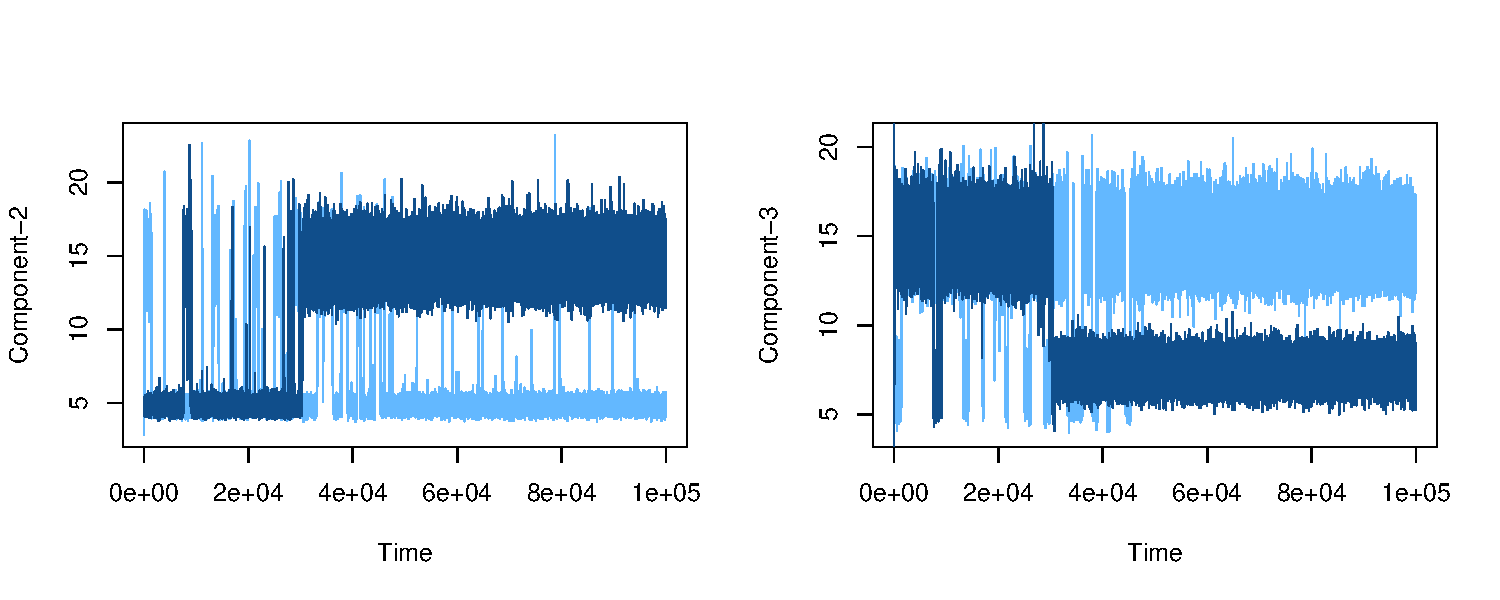
\includegraphics[width = 0.9\textwidth]{plots/poisson-trace_n1e+05.pdf}
    \caption{Trace plot for second (left) and third (right) component of two chains started from random points.The two colors denote the two different chains.}
    \label{fig:poisson-trace}
\end{figure}

This is a 7-dimensional estimation problem wherein the marginal distribution of majority of components display a multimodal nature. Figure~\ref{fig:poisson-trace} shows the evolution of two chains started from random points with time for the second component. We will report the ACF plots for component-2. Similar behavior is observed for ACF plots of other components as well.\\

\begin{figure}[h]
    \centering
    \begin{subfigure}[h]{.8\textwidth}
      \centering
      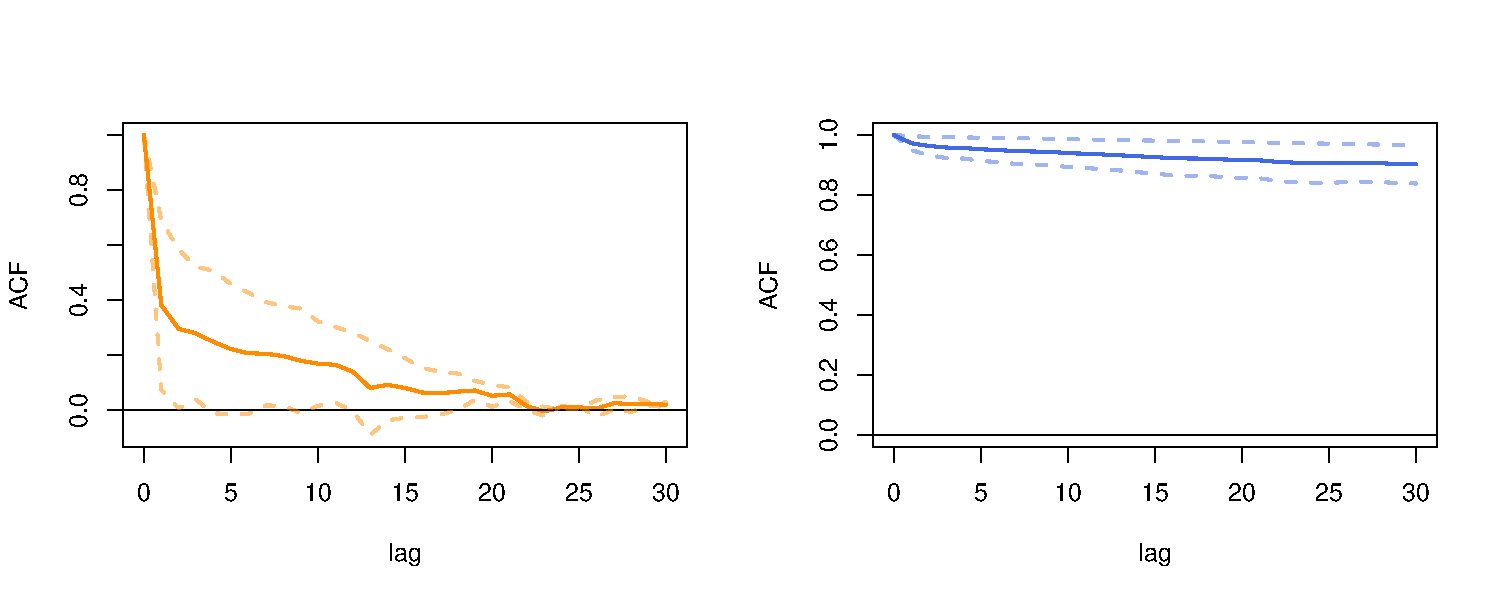
\includegraphics[width = \textwidth]{plots/poisson-acf_n1000.pdf}
      \caption{$n = 1000$}
      \label{subfig:poisson-acf_n1e3}
    \end{subfigure}
    \begin{subfigure}[h]{.8\textwidth}
      \centering
      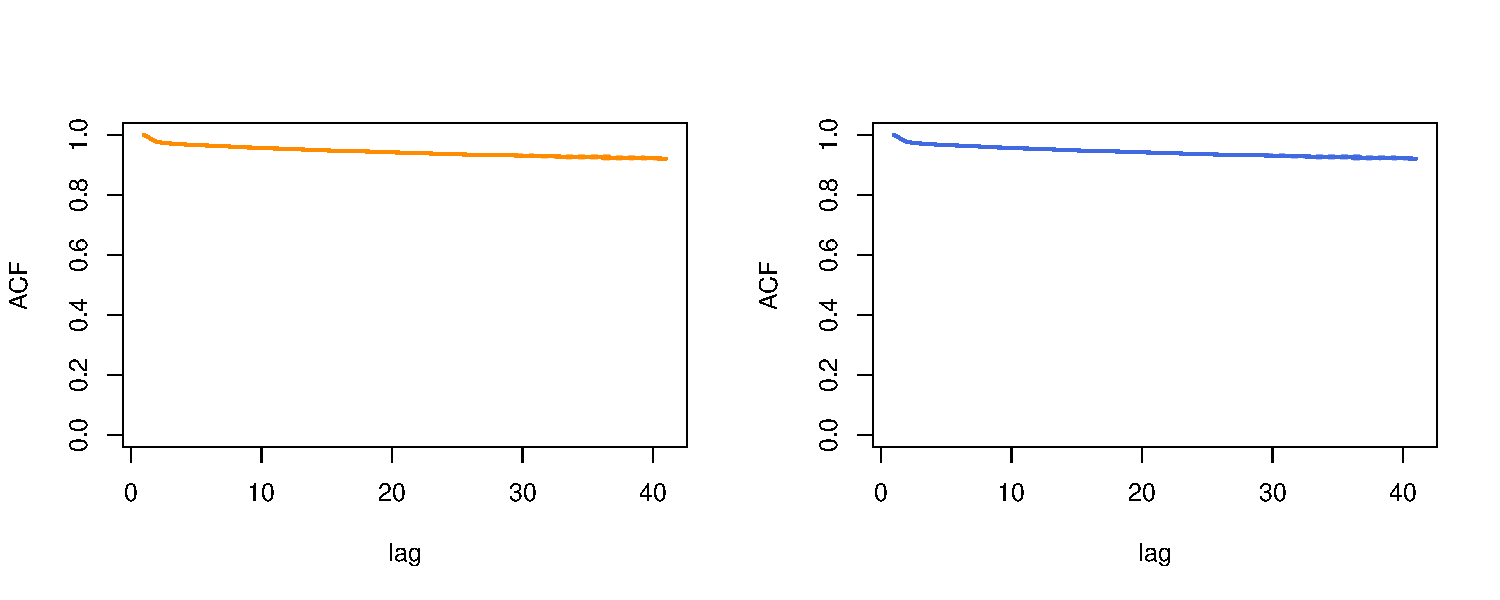
\includegraphics[width = \textwidth]{plots/poisson-acf_n10000.pdf}
      \caption{$n = 10000$}
      \label{subfig:poisson-acf_n1e4}
    \end{subfigure}
    \caption{Poisson change point. ACF (left) and G-ACF (right) for individual chains and average over $m$ chains for two chain lengths.}
    \label{fig:poisson-acf}
\end{figure}

Figure~\ref{fig:poisson-acf} demonstrates a striking advantage of G-ACF in estimating the true autocorrelations. G-ACF gives a more realistic and accurate estimation of autocorrelations in almost ten times lesser chain length.

 % it is evident that the chains have not explored the sample space well. Hence for $10^3$ samples ACF severely underestimates the autocorrelations whereas G-ACF gives more realistic estimates. For a large sample size of $10^5$, the Markov chains have mixed properly and therefore, both the estimators are approximately alike.

\subsection{Network crawling}

% \cite{handcock2008statnet} implemented an exponential-family random graph modelling (ERGM) on network data in the package . 

The \texttt{faux.magnolia.high} dataset available in the \texttt{ergm} \texttt{R} package represents a simulated within school friendship network based on Ad-Health data (\cite{resnick1997protecting}). The school communities represented by the network data are located in the southern United States. Each node represents a student and each edge represents a friendship between the nodes it connects.

The goal is to draw nodes uniformly from the network by using a network crawler. \cite{nilakanta2019ensuring} modified the data by removing 1,022 out of 1,461 nodes to obtain a well-connected graph. This resulting social network has 439 nodes and 573 edges. We use a Metropolis-Hastings algorithm with a simple random-walk  proposal suggested by \cite{gjoka2011practical}. Each node is associated with five features namely - degree of connection, cluster coefficient, grade, binary sex indicator (1 for female, 0 for male), and binary race indicator (1 for white, 0 for others).\\

\begin{figure}
    \centering
    \begin{subfigure}[h]{.8\textwidth}
      \centering
      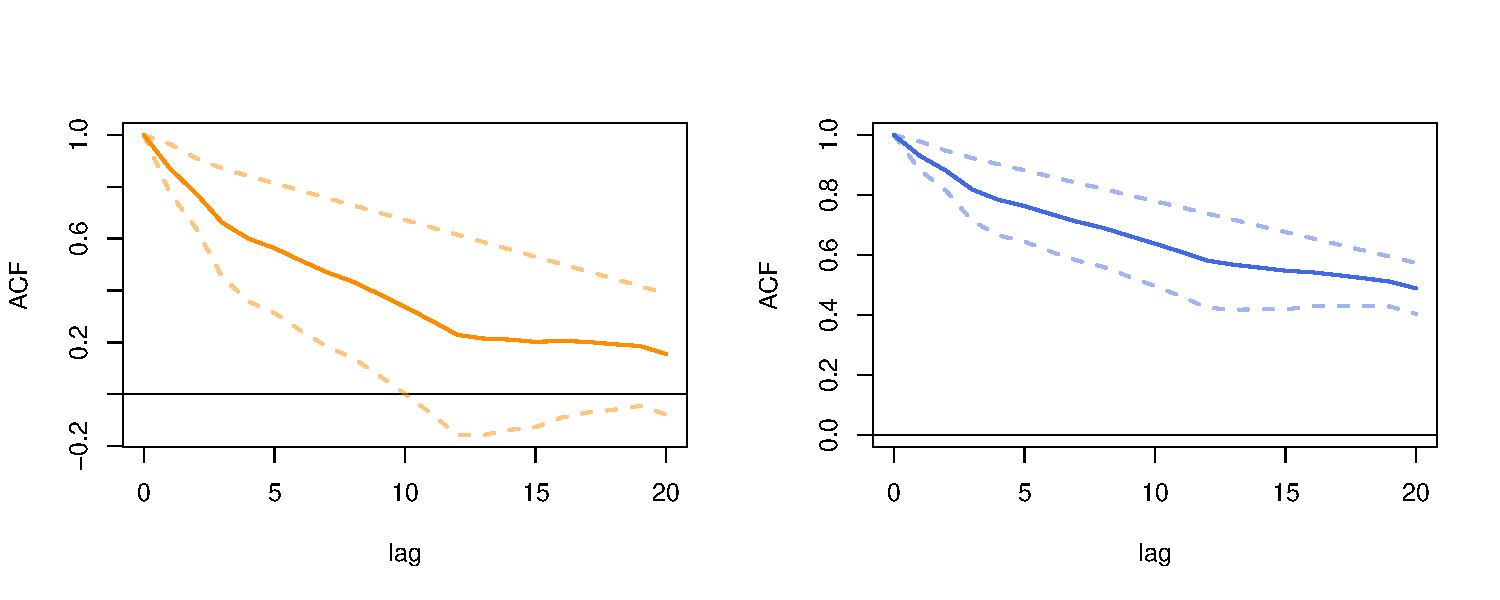
\includegraphics[width = \textwidth]{plots/magnolia-acf_n100.pdf}
      \caption{$n = 100$}
      \label{subfig:magnolia-acf_n1e3}
    \end{subfigure}
    \begin{subfigure}[h]{.8\textwidth}
      \centering
      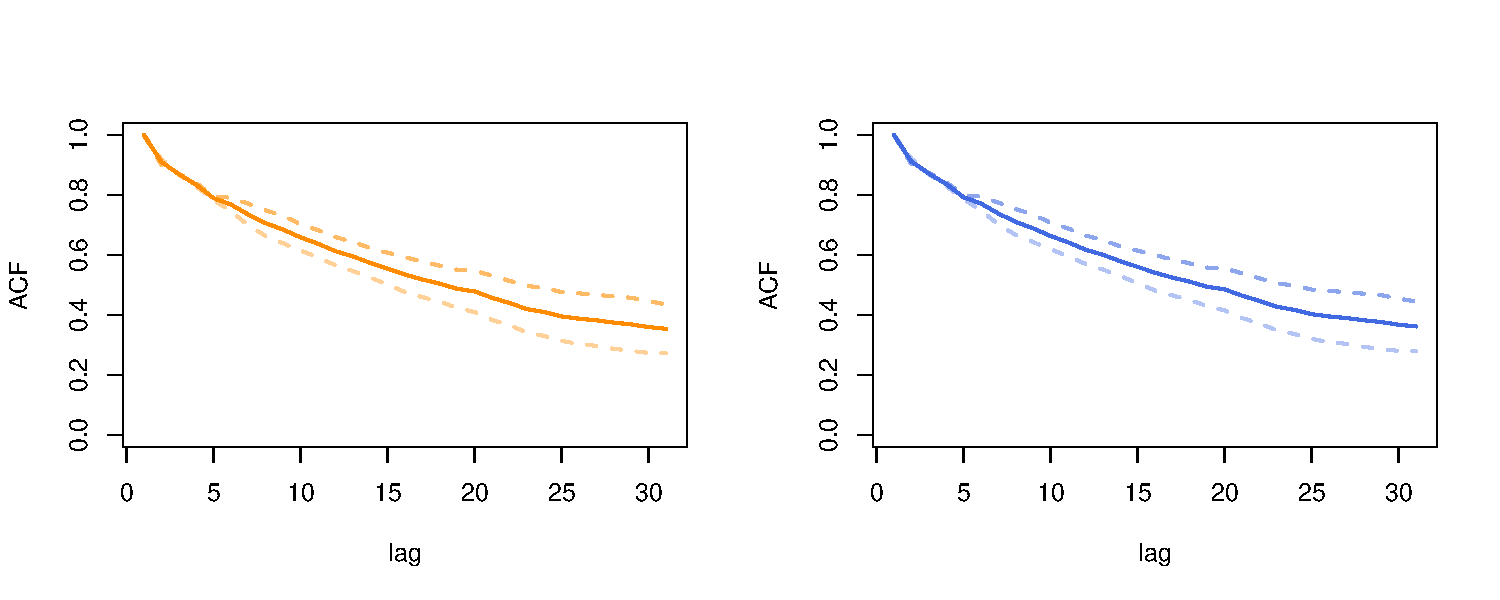
\includegraphics[width = \textwidth]{plots/magnolia-acf_n1000.pdf}
      \caption{$n = 1000$}
      \label{subfig:magnolia-acf_n1e4}
    \end{subfigure}
    \caption{Network crawling. ACF (left) and G-ACF (right) for individual chains and average over $m$ chains for two chain lengths.}
    \label{fig:magnolia-acf}
\end{figure}
% , i.e. $\lambda(i) = 1/n$ for all $i \in V$.  The Metropolis-Hastings transition kernel for this method is

% Let $V$ denote the non-empty set of countable nodes, $E \subseteq V \times V$ denote the set of edges, and $G = (V,E)$ denote the network. We are interested in exploring all the nodes uniformly, i.e. sample from a uniform distribution over $V$. Let $\lambda$ denote a uniform distribution over $V$  let $h: V \to \mathbb{R}^p$ map each node to certain features of interest. If $X \sim \lambda$, we wish to calculate the expected value of $h(X)$ with respect to $\lambda$ given by

% \[
% \mathbb{E}[h(X)]_{\lambda} = \dfrac{1}{n}\sum_{x \in V}h(x).
% \]

% Here n is the set cardinality of $V$. 



% \[
% P(i,j) = \begin{cases}
%              \dfrac{1}{d_i} \min\left\{1, d_i{d_j}^{-1}\right\} & \textrm{if $j$ is a neighbor of $i$}  \\
%              1 - \sum_{k \neq i} d_i^{-1} \min \left\{1, {d_i}{d_k}^{-1}\right\} & \textrm{if } j = i\\
%              0 & \textrm{otherwise}.
%         \end{cases}
% \]

% Table (blah) shows the population parameters we are interested in estimating using MCMC methods.  The race and sex parameters are estimated as proportion of whites and females in the sample respectively. 

We believe that the students from different races engage in a "selective networking" which might cause formation of clusters in the network wherein students within a cluster engage more with each other than with the students outside it. We sample two parallel Markov chains starting from two students belonging to different races and study its impacts on the average features of their immediate social group. Figure~\ref{fig:magnolia-acf} shows the ACF and G-ACF plots for the third feature at two different simulation sizes. As evident, G-ACF displays a clear advantage over ACF in just $n=100$ samples.

% It is hypothesized that students from certain communities tend to engage more with students of same or other marginally represented communities. We believe that this "selective networking" might cause formation of clusters in the network wherein students within a cluster engage more with each other than with the students outside it. Given that the graph is well-connected, the Markov chains will eventually explore all the nodes. 


\singlespacing
\bibliographystyle{apalike}
\bibliography{sample}
\end{document}
